\documentclass[twoside]{report}
\usepackage{url}

\usepackage[nottoc,numbib]{tocbibind}
%%%%%%%%%%%%%%%%%%%%%%%%%%%%%%%%%
% PACKAGE IMPORTS
%%%%%%%%%%%%%%%%%%%%%%%%%%%%%%%%%


\usepackage[tmargin=2cm,rmargin=1in,lmargin=1in,margin=0.85in,bmargin=2cm,footskip=.2in]{geometry} % I woulld suggest dont play with the margin. It kind of ruins the contents page.
\usepackage{amsmath,amsfonts,amsthm,amssymb,mathtools}
\usepackage{bookmark}
\usepackage[inline]{enumitem}
\usepackage{cancel}
\usepackage{hyperref,theoremref}
\hypersetup{
	colorlinks=true, linkcolor=doc!80, urlcolor=doc!80, citecolor=mydefinitfr!80!black,
	bookmarksnumbered=true,
	bookmarksopen=true
}
\usepackage[most,many,breakable]{tcolorbox}
\usepackage{xcolor}
\usepackage{graphicx}
\usepackage{changepage}
%\graphicspath{ {./images/} } %give your suitable image path
\usepackage{varwidth}
\usepackage{authblk}
\usepackage{marvosym}
\usepackage{nameref}
\usepackage{multicol,array,multirow}
\usepackage{tikz-cd}
\usepackage{cancel}
\usepackage{caption} 
\usepackage{pgfplots}
%\usepackage[Sonny]{fncychap}
\usepackage{mathrsfs} 
\usepackage{bbm}
\usepackage[ruled,vlined,linesnumbered]{algorithm2e}
\usepackage{fancyhdr}
\usepackage{optidef}
%\pagestyle{fancy}
\fancypagestyle{plain}{%
	\renewcommand{\headrulewidth}{0pt}%
	\fancyhf{}%
}
\fancypagestyle{fancy}{
\fancyhead{}
\renewcommand{\headrulewidth}{1pt}
\fancyhead[LE]{\itshape\textsc{\nouppercase\rightmark}}
\fancyhead[RO]{\itshape\textsc\leftmark} % CO Centered Odd
\fancyfoot{}
\fancyhead[RE,LO]{\itshape Page \thepage}
}
\makeatletter
\renewcommand{\chaptermark}[1]{%
  \markboth{%
    \ifnum\c@secnumdepth>\m@ne
      \@chapapp\ {\thechapter} \ %
    \fi
  #1%
  }{}%
}
\def\sectionmark#1{%
    \markright {\MakeUppercase{%
      \ifnum \c@secnumdepth >\z@
        \thesection \ %
      \fi
      #1}}}
\makeatother

\DeclareMathOperator{\supp}{supp}
\DeclareMathOperator{\rk}{Rank}
\DeclareMathOperator{\conv}{Conv}
\DeclareMathOperator{\pne}{\mathsf{PNE}}
\DeclareMathOperator{\mne}{\mathsf{MNE}}
\DeclareMathOperator{\cce}{\mathsf{CCE}}
\DeclareMathOperator{\ce}{\mathsf{CE}}
\DeclareMathOperator{\poa}{\mathsf{PoA}}
\DeclareMathOperator{\pls}{\mathsf{PLS}}
\DeclareMathOperator{\brd}{\mathsf{BRD}}


%%%%%%%%%%%%%%%%%%%%%%%%%%%%%%%%%%%%%
% FONT SETS
%%%%%%%%%%%%%%%%%%%%%%%%%%%%%%%%%%%%%

%%%%%%%%%%%%%%% SET 1 %%%%%%%%%%%%%%%

%\usepackage[T1]{fontenc}
%\usepackage{baskervald}  % Baskerville-like font
%\usepackage[scaled]{beramono}  % Optional: better monospaced font
%\usepackage[utopia]{newtxmath} % Match with Utopia-like math

%%%%%%%%%%%%%%% SET 2 %%%%%%%%%%%%%%%

%\usepackage[T1]{fontenc}  % Ensure proper font encoding
%\usepackage{erewhon}      % Use Erewhon (Utopia-based) for text
%\usepackage[utopia]{newtxmath} % Use Utopia-compatible math fonts

%%%%%%%%%%%%%%% SET 3 %%%%%%%%%%%%%%%

\usepackage[T1]{fontenc}   % Proper font encoding
\usepackage{XCharter}      % XCharter for the main text
\usepackage[varqu,varl]{inconsolata} % Optional: Better monospaced font
\usepackage[charter]{newtxmath} % Use newtxmath with Charter-compatible math

%%%%%%%%%%%%%%% SET 4 %%%%%%%%%%%%%%%

%\usepackage{mathpazo}
%\usepackage{libertine}
%\usepackage[libertine]{newtxmath}


%%%%%%%%%%%%%%%%%%%%%%%%%%%%%%
% SELF MADE COLORS
%%%%%%%%%%%%%%%%%%%%%%%%%%%%%%

\usetikzlibrary{ shapes.geometric }
\usetikzlibrary{calc}
\usepackage{anyfontsize}
\definecolor{doc}{RGB}{0,60,110}
\definecolor{myg}{RGB}{56, 140, 70}
\definecolor{myb}{RGB}{45, 111, 177}
\definecolor{myr}{RGB}{199, 68, 64}
\definecolor{mybg}{HTML}{F2F2F9}
\definecolor{mytheorembg}{HTML}{F2F2F9}
\definecolor{mytheoremfr}{HTML}{00007B}
\definecolor{myexamplebg}{HTML}{F2FBF8}
\definecolor{myexamplefr}{HTML}{88D6D1}
\definecolor{myexampleti}{HTML}{2A7F7F}
\definecolor{mydefinitbg}{HTML}{E5E5FF}
\definecolor{mydefinitfr}{HTML}{3F3FA3}
\definecolor{notesgreen}{RGB}{0,162,0}
\definecolor{myp}{RGB}{197, 92, 212}
\definecolor{mygr}{HTML}{2C3338}
\definecolor{myred}{RGB}{127,0,0}
\definecolor{myyellow}{RGB}{169,121,69}
\definecolor{OrangeRed}{HTML}{ED135A}
\definecolor{Dandelion}{HTML}{FDBC42}
\definecolor{light-gray}{gray}{0.95}
\definecolor{Emerald}{HTML}{00A99D}
\definecolor{RoyalBlue}{HTML}{0071BC}
\definecolor{mytoccolor}{HTML}{886830}

\renewcommand{\qed}{\ensuremath{\blacksquare}}

%\newcommand{\bfs}{basic feasible solution}
%\usepackage{fontspec}

% Load the custom font and create a command \useabcfont{}
%\newfontface\abcfont{Letter Gothic MT Std Regular.otf}

%\newcommand{\useabcfont}[1]{{\abcfont #1}}
%%%%%%%%%%%%%%%%%%%%%%%%%%%%
% TCOLORBOX SETUPS
%%%%%%%%%%%%%%%%%%%%%%%%%%%%

\setlength{\parindent}{1cm}
%================================
% THEOREM BOX
%================================

\tcbuselibrary{theorems,skins,hooks}
\newtcbtheorem[number within=section]{Theorem}{Theorem}
{%
	enhanced,
	breakable,
	colback = mytheorembg,
	frame hidden,
	boxrule = 0sp,
	borderline west = {2pt}{0pt}{mytheoremfr},
	sharp corners,
	detach title,
	before upper = \tcbtitle\par\smallskip,
	coltitle = mytheoremfr,
	fonttitle = \bfseries\sffamily,
	description font = \mdseries,
	separator sign none,
	segmentation style={solid, mytheoremfr},
}
{th}

\tcbuselibrary{theorems,skins,hooks}
\newtcbtheorem[number within=chapter]{theorem}{Theorem}
{%
	enhanced,
	breakable,
	colback = mytheorembg,
	frame hidden,
	boxrule = 0sp,
	borderline west = {2pt}{0pt}{mytheoremfr},
	sharp corners,
	detach title,
	before upper = \tcbtitle\par\smallskip,
	coltitle = mytheoremfr,
	fonttitle = \bfseries\sffamily,
	description font = \mdseries,
	separator sign none,
	segmentation style={solid, mytheoremfr},
}
{th}


\tcbuselibrary{theorems,skins,hooks}
\newtcolorbox{Theoremcon}
{%
	enhanced
	,breakable
	,colback = mytheorembg
	,frame hidden
	,boxrule = 0sp
	,borderline west = {2pt}{0pt}{mytheoremfr}
	,sharp corners
	,description font = \mdseries
	,separator sign none
}


%================================
% Corollery
%================================
\tcbuselibrary{theorems,skins,hooks}
\newtcbtheorem[use counter from=Theorem, number within=section]{corolary}{Corollary}
{%
	enhanced
	,breakable
	,colback = myp!10
	,frame hidden
	,boxrule = 0sp
	,borderline west = {2pt}{0pt}{myp!60!black}
	,sharp corners
	,detach title
	,before upper = \tcbtitle\par\smallskip
	,coltitle = myp!60!black
	,fonttitle = \bfseries\sffamily
	,description font = \mdseries
	,separator sign none
	,segmentation style={solid, myp!85!black}
%	enhanced
%	,breakable
%	,colback = mytheorembg
%	,frame hidden
%	,boxrule = 0sp
%	,borderline west = {2pt}{0pt}{mytheoremfr}
%	,sharp corners
%	,detach title
%	,before upper = \tcbtitle\par\smallskip
%	,coltitle = mytheoremfr
%	,fonttitle = \bfseries\sffamily
%	,description font = \mdseries
%	,separator sign none
%	,segmentation style={solid, mytheoremfr}
}
{th}
\tcbuselibrary{theorems,skins,hooks}
\newtcbtheorem[use counter from=theorem, number within=chapter]{corollary}{Corollary}
{%
	enhanced
	,breakable
	,colback = mytheorembg
	,frame hidden
	,boxrule = 0sp
	,borderline west = {2pt}{0pt}{myp!60!black}
	,sharp corners
	,detach title
	,before upper = \tcbtitle\par\smallskip
	,coltitle = myp!60!black
	,fonttitle = \bfseries\sffamily
	,description font = \mdseries
	,separator sign none
	,segmentation style={solid, myp!85!black}
}
{th}

%================================
% LEMMA
%================================

\tcbuselibrary{theorems,skins,hooks}
\newtcbtheorem[use counter from=Theorem, number within=section]{lemma}{Lemma}
{%
	enhanced
	,breakable
	,colback = myg!10
	,frame hidden
	,boxrule = 0sp
	,borderline west = {2pt}{0pt}{myg}
	,sharp corners
	,detach title
	,before upper = \tcbtitle\par\smallskip
	,coltitle = myg!85!black
	,fonttitle = \bfseries\sffamily
	,description font = \mdseries
	,separator sign none
	,segmentation style={solid, myg!85!black}
}
{th}


\newtcbtheorem[use counter from=theorem, number within=chapter]{Lemma}{Lemma}
{%
	enhanced
	,breakable
	,colback = myg!10
	,frame hidden
	,boxrule = 0sp
	,borderline west = {2pt}{0pt}{myg}
	,sharp corners
	,detach title
	,before upper = \tcbtitle\par\smallskip
	,coltitle = myg!85!black
	,fonttitle = \bfseries\sffamily
	,description font = \mdseries
	,separator sign none
	,segmentation style={solid, myg!85!black}
}
{th}

%================================
% CLAIM
%================================

\tcbuselibrary{theorems,skins,hooks}
\newtcbtheorem[use counter from=Theorem, number within=section]{claim}{Claim}
{%
	enhanced
	,breakable
	,colback = myg!10
	,frame hidden
	,boxrule = 0sp
	,borderline west = {2pt}{0pt}{myg}
	,sharp corners
	,detach title
	,before upper = \tcbtitle\par\smallskip
	,coltitle = myg!85!black
	,fonttitle = \bfseries\sffamily
	,description font = \mdseries
	,separator sign none
	,segmentation style={solid, myg!85!black}
}
{th}


\newtcbtheorem[use counter from=theorem, number within=chapter]{Claim}{Claim}
{%
	enhanced
	,breakable
	,colback = myg!10
	,frame hidden
	,boxrule = 0sp
	,borderline west = {2pt}{0pt}{myg}
	,sharp corners
	,detach title
	,before upper = \tcbtitle\par\smallskip
	,coltitle = myg!85!black
	,fonttitle = \bfseries\sffamily
	,description font = \mdseries
	,separator sign none
	,segmentation style={solid, myg!85!black}
}
{th}

%================================
% EXAMPLE BOX
%================================

\newtcbtheorem[number within=section]{Example}{Example}
{%
	colback = myexamplebg
	,breakable
	,colframe = myexamplefr
	,coltitle = myexampleti
	,boxrule = 1pt
	,sharp corners
	,detach title
	,before upper=\tcbtitle\par\smallskip
	,fonttitle = \bfseries
	,description font = \mdseries
	,separator sign none
	,description delimiters parenthesis
}
{ex}

\newtcbtheorem[number within=chapter]{example}{Example}
{%
	colback = myexamplebg
	,breakable
	,colframe = myexamplefr
	,coltitle = myexampleti
	,boxrule = 1pt
	,sharp corners
	,detach title
	,before upper=\tcbtitle\par\smallskip
	,fonttitle = \bfseries
	,description font = \mdseries
	,separator sign none
	,description delimiters parenthesis
}
{ex}

%================================
% DEFINITION BOX
%================================

\newtcbtheorem[number within=section]{Definition}{Definition}{enhanced,
	before skip=2mm,after skip=2mm, colback=red!5,colframe=red!80!black,boxrule=0.5mm,
	attach boxed title to top left={xshift=1cm,yshift*=1mm-\tcboxedtitleheight}, varwidth boxed title*=-3cm,colbacktitle=red!75!black,
	boxed title style={frame code={
			\path[fill=tcbcolback]
			([yshift=-1mm,xshift=-1mm]frame.north west)
			arc[start angle=0,end angle=180,radius=1mm]
			([yshift=-1mm,xshift=1mm]frame.north east)
			arc[start angle=180,end angle=0,radius=1mm];
			\path[left color=tcbcolback!60!black,right color=tcbcolback!60!black,
			middle color=tcbcolback!80!black]
			([xshift=-2mm]frame.north west) -- ([xshift=2mm]frame.north east)
			[rounded corners=1mm]-- ([xshift=1mm,yshift=-1mm]frame.north east)
			-- (frame.south east) -- (frame.south west)
			-- ([xshift=-1mm,yshift=-1mm]frame.north west)
			[sharp corners]-- cycle;
		},interior engine=empty,
	},
	fonttitle=\bfseries,
	title={#2},#1}{def}
\newtcbtheorem[number within=chapter]{definition}{Definition}{enhanced,
	before skip=2mm,after skip=2mm, colback=red!5,colframe=red!80!black,boxrule=0.5mm,
	attach boxed title to top left={xshift=1cm,yshift*=1mm-\tcboxedtitleheight}, varwidth boxed title*=-3cm, colbacktitle=red!75!black,
	boxed title style={frame code={
			\path[fill=red!75!black]
			([yshift=-1mm,xshift=-1mm]frame.north west)
			arc[start angle=0,end angle=180,radius=1mm]
			([yshift=-1mm,xshift=1mm]frame.north east)
			arc[start angle=180,end angle=0,radius=1mm];
			\path[left color=tcbcolback!60!black,right color=tcbcolback!60!black,
			middle color=tcbcolback!80!black]
			([xshift=-2mm]frame.north west) -- ([xshift=2mm]frame.north east)
			[rounded corners=1mm]-- ([xshift=1mm,yshift=-1mm]frame.north east)
			-- (frame.south east) -- (frame.south west)
			-- ([xshift=-1mm,yshift=-1mm]frame.north west)
			[sharp corners]-- cycle;
		},interior engine=empty,
	},
	fonttitle=\bfseries,
	title={#2},#1}{def}


%================================
% OPEN QUESTION BOX
%================================

\newtcbtheorem[number within=section]{open}{Open Question}{enhanced,
	before skip=2mm,after skip=2mm, colback=myp!5,colframe=myp!80!black,boxrule=0.5mm,
	attach boxed title to top left={xshift=1cm,yshift*=1mm-\tcboxedtitleheight}, varwidth boxed title*=-3cm, colbacktitle=myp!75!black,
	boxed title style={frame code={
			\path[fill=tcbcolback]
			([yshift=-1mm,xshift=-1mm]frame.north west)
			arc[start angle=0,end angle=180,radius=1mm]
			([yshift=-1mm,xshift=1mm]frame.north east)
			arc[start angle=180,end angle=0,radius=1mm];
			\path[left color=tcbcolback!60!black,right color=tcbcolback!60!black,
			middle color=tcbcolback!80!black]
			([xshift=-2mm]frame.north west) -- ([xshift=2mm]frame.north east)
			[rounded corners=1mm]-- ([xshift=1mm,yshift=-1mm]frame.north east)
			-- (frame.south east) -- (frame.south west)
			-- ([xshift=-1mm,yshift=-1mm]frame.north west)
			[sharp corners]-- cycle;
		},interior engine=empty,
	},
	fonttitle=\bfseries,
	title={#2},#1}{def}
\newtcbtheorem[number within=chapter]{Open}{Open Question}{enhanced,
	before skip=2mm,after skip=2mm, colback=myp!5,colframe=myp!80!black,boxrule=0.5mm,
	attach boxed title to top left={xshift=1cm,yshift*=1mm-\tcboxedtitleheight}, varwidth boxed title*=-3cm, colbacktitle=myp!75!black,
	boxed title style={frame code={
			\path[fill=tcbcolback]
			([yshift=-1mm,xshift=-1mm]frame.north west)
			arc[start angle=0,end angle=180,radius=1mm]
			([yshift=-1mm,xshift=1mm]frame.north east)
			arc[start angle=180,end angle=0,radius=1mm];
			\path[left color=tcbcolback!60!black,right color=tcbcolback!60!black,
			middle color=tcbcolback!80!black]
			([xshift=-2mm]frame.north west) -- ([xshift=2mm]frame.north east)
			[rounded corners=1mm]-- ([xshift=1mm,yshift=-1mm]frame.north east)
			-- (frame.south east) -- (frame.south west)
			-- ([xshift=-1mm,yshift=-1mm]frame.north west)
			[sharp corners]-- cycle;
		},interior engine=empty,
	},
	fonttitle=\bfseries,
	title={#2},#1}{def}



%================================
% EXERCISE BOX
%================================

\makeatletter
\newtcbtheorem[number within=chapter]{problem}{Problem}{enhanced,
	breakable,
	colback=white,
	colframe=myb!80!black,
	attach boxed title to top left={yshift*=-\tcboxedtitleheight},
	fonttitle=\bfseries,
	title={#2},
	boxed title size=title,
	boxed title style={%
		sharp corners,
		rounded corners=northwest,
		colback=tcbcolframe,
		boxrule=0pt,
	},
	underlay boxed title={%
		\path[fill=tcbcolframe] (title.south west)--(title.south east)
		to[out=0, in=180] ([xshift=5mm]title.east)--
		(title.center-|frame.east)
		[rounded corners=\kvtcb@arc] |-
		(frame.north) -| cycle;
	},
	#1
}{def}
\makeatother


%================================
% Question BOX
%================================


\makeatletter
\newtcbtheorem[number within=chapter]{question}{Question}{enhanced,
	breakable,
	colback=white,
	colframe=myb!80!black,
	attach boxed title to top left={yshift*=-\tcboxedtitleheight},
	fonttitle=\bfseries,
	title={#2},
	boxed title size=title,
	boxed title style={%
		sharp corners,
		rounded corners=northwest,
		colback=tcbcolframe,
		boxrule=0pt,
	},
	underlay boxed title={%
		\path[fill=tcbcolframe] (title.south west)--(title.south east)
		to[out=0, in=180] ([xshift=5mm]title.east)--
		(title.center-|frame.east)
		[rounded corners=\kvtcb@arc] |-
		(frame.north) -| cycle;
	},
	#1
}{qs}
\makeatother

\newtcbtheorem[number within=chapter]{wconc}{Wrong Concept}{
	breakable,
	enhanced,
	colback=white,
	colframe=myr,
	arc=0pt,
	outer arc=0pt,
	fonttitle=\bfseries\sffamily\large,
	colbacktitle=myr,
	attach boxed title to top left={},
	boxed title style={
		enhanced,
		skin=enhancedfirst jigsaw,
		arc=3pt,
		bottom=0pt,
		interior style={fill=myr}
	},
	#1
}{def}



%================================
% NOTE BOX
%================================

\usetikzlibrary{arrows,calc,shadows.blur}
\tcbuselibrary{skins}
\newtcolorbox{note}[1][]{%
	enhanced jigsaw,
	colback=gray!20!white,%
	colframe=gray!80!black,
	size=small,
	boxrule=1pt,
	title=\textbf{Note:-},
	halign title=flush center,
	coltitle=black,
	breakable,
	drop shadow=black!50!white,
	attach boxed title to top left={xshift=1cm,yshift=-\tcboxedtitleheight/2,yshifttext=-\tcboxedtitleheight/2},
	minipage boxed title=1.5cm,
	boxed title style={%
		colback=white,
		size=fbox,
		boxrule=1pt,
		boxsep=2pt,
		underlay={%
			\coordinate (dotA) at ($(interior.west) + (-0.5pt,0)$);
			\coordinate (dotB) at ($(interior.east) + (0.5pt,0)$);
			\begin{scope}
				\clip (interior.north west) rectangle ([xshift=3ex]interior.east);
				\filldraw [white, blur shadow={shadow opacity=60, shadow yshift=-.75ex}, rounded corners=2pt] (interior.north west) rectangle (interior.south east);
			\end{scope}
			\begin{scope}[gray!80!black]
				\fill (dotA) circle (2pt);
				\fill (dotB) circle (2pt);
			\end{scope}
		},
	},
	#1,
}

%================================
% Algorithm Problem Definition
%================================

\makeatletter
\usepackage{tabularx,environ}
\newcommand{\problemtitle}[1]{\gdef\@problemtitle{\scshape #1}}% Store problem title
\newcommand{\probleminput}[1]{\gdef\@probleminput{#1}}% Store problem input
\newcommand{\problemquestion}[1]{\gdef\@problemquestion{#1}}% Store problem question
\NewEnviron{algoprob}{
	\problemtitle{}\probleminput{}\problemquestion{}% Default input is empty
	\BODY% Parse input
	\par\addvspace{.5\baselineskip}
	\noindent
	\begin{tabularx}{\textwidth}{@{\hspace{\parindent}} l X c}
		\multicolumn{2}{@{\hspace{\parindent}}l}{\@problemtitle} \\% Title
		\textbf{Input:} & \@probleminput \\% Input
		\textbf{Question:} & \@problemquestion% Question
	\end{tabularx}
	\par\addvspace{.5\baselineskip}
}
\makeatother


%%%%%%%%%%%%%%%%%%%%%%%%%%%%%%
% SELF MADE COMMANDS
%%%%%%%%%%%%%%%%%%%%%%%%%%%%%%

%% The environments which are appears in pairs one of them is for the chapters which have sections whose environment name starts with small letter and the other is for chapters which do not have sections whose environment name starts with capital letter. In the short command for the latter I used the letter 'c' to represent it should be use if it is not under a section

%% Short commands for environments goes like this
%% \<command name>[<reference name>]{<heading>}{<description>}
%% For example in theorem for suppose Fundamental Theorem of Calculus i will write like this
%% \thm[ftc]{Fundamental Theorem of Calculus}{Theorem Statement}

\NewDocumentCommand{\EqM}{ m O{black} m}{%
	\tikz[remember picture, baseline, anchor=base] 
	\node[inner sep=0pt, outer sep=3pt, text=#2] (#1) {%
		\ensuremath{#3}%
	};    
}



\newcommand{\thm}[3][]{\begin{Theorem}{#2}{#1}#3\end{Theorem}}
\newcommand{\thmc}[3][]{\begin{theorem}{#2}{#1}#3\end{theorem}}
\newcommand{\cor}[3][]{\begin{corolary}{#2}{#1}#3\end{corolary}}
\newcommand{\corc}[3][]{\begin{corollary}{#2}{#1}#3\end{corollary}}
\newcommand{\lem}[3][]{\begin{lemma}{#2}{#1}#3\end{lemma}}
\newcommand{\clm}[3][]{\begin{claim}{#2}{#1}#3\end{claim}}
\newcommand{\wc}[3][]{\begin{wconc}{#2}{#1}\setlength{\parindent}{1cm}#3\end{wconc}}
\newcommand{\thmcon}[1]{\begin{Theoremcon}{#1}\end{Theoremcon}}
\newcommand{\ex}[3][]{\begin{Example}{#2}{#1}#3\end{Example}}
\newcommand{\exc}[3][]{\begin{example}{#2}{#1}#3\end{example}}
\newcommand{\dfn}[3][]{\begin{Definition}{#2}{#1}#3\end{Definition}}
\newcommand{\dfnc}[3][]{\begin{definition}{#2}{#1}#3\end{definition}}
\newcommand{\opn}[3][]{\begin{open}{#2}{#1}#3\end{open}}
\newcommand{\opnc}[3][]{\begin{Open}{#2}{#1}#3\end{Open}}
\newcommand{\pr}[3][]{\begin{problem}{#2}{#1}#3\end{problem}}





\newtheorem*{observation*}{Observation}
\newtheorem*{idea*}{Idea}
\newtheorem*{assumption*}{Assumption}
\newtheorem{observation}{Observation}[chapter]
\newtheorem{fact}[observation]{Fact}
\newtheorem{assumption}{Assumption}[chapter]


\renewenvironment{proof}{\noindent{\textit{\textbf{Proof:}}}\hspace*{1em}}{\hfill\qed\bigskip\\}
\newenvironment{combi-proof}{\noindent{\textbf{\textit{Combinatorial Proof:}}}\hspace*{1em}}{\hfill\qed\bigskip\\}
\newenvironment{alg-proof}{\noindent{\textbf{\textit{Algebraic Proof:}}}\hspace*{1em}}{\hfill\qed\bigskip\\}
\newenvironment{proof-sketch}{\noindent{\textbf{\textit{Sketch of Proof:}}}\hspace*{1em}}{\hfill\qed\bigskip\\}
\newenvironment{proof-idea}{\noindent{\textbf{\textit{Proof Idea:}}}\hspace*{1em}}{\hfill\qed\bigskip\\}
\newenvironment{proof-of-theorem}[1][]{\noindent{\textbf{\textit{Proof of \thmref{#1}:}}}\hspace*{1em}}{\hfill\qed\bigskip\\}
\newenvironment{proof-of-lemma}[1][]{\noindent{\textbf{\textit{Proof of  \lmref{#1}:}}}\hspace*{1em}}{\hfill\qed\bigskip\\}
\newenvironment{proof-of-corollary}[1][]{\noindent{\textbf{\textit{Proof of \corrref{#1}:}}}\hspace*{1em}}{\hfill\qed\bigskip\\}
\newenvironment{proof-attempt}{\noindent{\textbf{\textit{Proof Attempt:}}}\hspace*{1em}}{\hfill\qed\bigskip\\}
\newenvironment{alternate-proof}[1][]{\noindent{\textit{\textbf{Alternate Proof #1:}}}\hspace*{1em}}{\hfill\qed\bigskip\\}
\newenvironment{proofof}[1]{\noindent{\textbf{\textit{Proof:
	of #1:}}}\hspace*{1em}}{\hfill\qed\bigskip\\}
\newenvironment{remark}{\noindent{Remark:}\hspace*{1em}}{\bigskip\\}
\newenvironment{idea}{\noindent{Idea: }}{\bigskip\\}



%% The proof environment actually multipurpose. For a proof many things actually play. Proof idea. Proof overview. Main pproof. Proof prerequisites etc. Thats why the first option uses the actual name of what exactly we are writing for the proof. It will go like this
%% Proof idea: \pf{Proof Idea}{content..}
%% Proof Overview: \pf{Proof Overview}{content..}
%% Proof : \pf{Proof}{content..}


\newcommand{\nt}[1]{\begin{note}#1\end{note}}

\newcommand*\circled[1]{\tikz[baseline=(char.base)]{
		\node[shape=circle,draw,inner sep=1pt] (char) {#1};}}
\newcommand\getcurrentref[1]{%
	\ifnumequal{\value{#1}}{0}
	{??}
	{\the\value{#1}}%
}

\newcounter{mylabelcounter}



\makeatletter
\newcommand{\setword}[2]{%
	\phantomsection
	#1\def\@currentlabel{\unexpanded{#1}}\label{#2}%
}
\makeatother


\tikzset{
	symbol/.style={
		draw=none,
		every to/.append style={
			edge node={node [sloped, allow upside down, auto=false]{$#1$}}}
	}
}


%%%%%%%%%%%%%%%%%%%%%%%%%%%%%%%%%%%%%%%%%%%
% TABLE OF CONTENTS 1
%%%%%%%%%%%%%%%%%%%%%%%%%%%%%%%%%%%%%%%%%%%
%
%\usepackage{framed}
%\usepackage{titletoc}
%\usepackage{etoolbox}
%\usepackage{lmodern}
%
%
%\patchcmd{\tableofcontents}{\contentsname}{\sffamily\contentsname}{}{}
%
%\renewenvironment{leftbar}
%{\def\FrameCommand{\hspace{6em}%
%				{\color{myyellow}\vrule width 2pt depth 6pt}\hspace{1em}}%
%		\MakeFramed{\parshape 1 0cm \dimexpr\textwidth-6em\relax\FrameRestore}\vskip2pt%
%	}
%{\endMakeFramed}
%
%\titlecontents{chapter}
%[0em]{\vspace*{2\baselineskip}}
%{\parbox{4.5em}{%
%				\hfill\Huge\sffamily\bfseries\color{myred}\thecontentspage}%
%		\vspace*{-2.3\baselineskip}\leftbar\textsc{\small\chaptername~\thecontentslabel}\\\sffamily}
%{}{\endleftbar}
%\titlecontents{section}
%[8.4em]
%{\sffamily\contentslabel{3em}}{}{}
%{\hspace{0.5em}\nobreak\itshape\color{myred}\contentspage}
%\titlecontents{subsection}
%[8.4em]
%{\sffamily\contentslabel{3em}}{}{}  
%{\hspace{0.5em}\nobreak\itshape\color{myred}\contentspage}



%%%%%%%%%%%%%%%%%%%%%%%%%%%%%%%%%%%%%%%%%%%
% TABLE OF CONTENTS 2
%%%%%%%%%%%%%%%%%%%%%%%%%%%%%%%%%%%%%%%%%%%


\usepackage{tikz}
\usetikzlibrary{shapes, positioning}
\usepackage{titletoc,titlesec}
\contentsmargin{0cm}
\setcounter{tocdepth}{3}
\setcounter{secnumdepth}{3}
\titlecontents{chapter}[3.7pc]
{\addvspace{30pt}%
	\begin{tikzpicture}[remember picture, overlay]%
		\draw[fill=mytoccolor,draw=mytoccolor] (-7,-.1) rectangle (-0.6,.5);%
		\pgftext[left,x=-3.6cm,y=0.2cm]{\color{white}\Large\sc\bfseries Chapter\ \thecontentslabel};%
	\end{tikzpicture}\color{mytoccolor}\large\sc\bfseries}%
{}
{}
{\;\titlerule\;\large\sc\bfseries Page \thecontentspage
	\begin{tikzpicture}[remember picture, overlay]
		\draw[fill=mytoccolor,draw=mytoccolor] (2pt,0) rectangle (4,0.1pt);
\end{tikzpicture}}%
\titlecontents{section}[3.7pc]
{\addvspace{2pt}}
{\contentslabel[\textcolor{mytoccolor}{\thecontentslabel}]{2pc}}
{}
{\hfill\small \textcolor{mytoccolor}{\thecontentspage}}
[]
\titlecontents{subsection}[3.7pc]
{\addvspace{-1pt}\small}
{\hspace*{2pc}\contentslabel[\textcolor{mytoccolor}{\thecontentslabel}]{2pc}}
{}
{\hfill\small \textcolor{mytoccolor}{\thecontentspage}}
[]
\titlecontents{subsubsection}[3.7pc]
{\addvspace{-1pt}\small}
{\hspace*{4.5pc}\contentslabel[\textcolor{mytoccolor}{\thecontentslabel}]{2.5pc}}
{}
{\hfill\small \textcolor{mytoccolor}{\thecontentspage}}
[]
% Adjust horizontal shift for subsubsections
%\titlecontents{subsubsection}[3.7pc]
%{\addvspace{-1pt}\small}
%{\hspace*{4pc}\contentslabel[\thecontentslabel]{2pc}} % Increase the hspace for a bigger horizontal shift
%{}
%{\hfill\small \thecontentspage}
%[]



\makeatletter
\renewcommand{\tableofcontents}{%
	\chapter*{%
		\vspace*{-80\p@}%
		\begin{tikzpicture}[remember picture, overlay]%
			\pgftext[right,x=15cm,y=0.2cm]{\color{mytoccolor}\Huge\sc\bfseries \contentsname};%
			\draw[fill=mytoccolor,draw=mytoccolor] (13,-.75) rectangle (20,1);%
			\clip (13,-.75) rectangle (20,1);
			\pgftext[right,x=15cm,y=0.2cm]{\color{white}\Huge\sc\bfseries \contentsname};%
	\end{tikzpicture}}%
	\@starttoc{toc}}
\makeatother
%\titleformat{\chapter}[display]
%{\normalfont\Huge\bfseries}{\chaptertitlename\ \thechapter}{20pt}{\Huge}


\newcommand\colorlink[3]{\href{#2}{\color{#1}#3}}
\newcommand\colorurl[2]{{\color{#1}\url{#2}}}

%%%%%%%%%%%%%%%%%%%%%%%%%%%%%%%%%%%%%%%%%%%
% Title Page 1
%%%%%%%%%%%%%%%%%%%%%%%%%%%%%%%%%%%%%%%%%%%

\newcommand{\mytitlea}[4]{
	\begin{tikzpicture}[remember picture,overlay]
		%%%%%%%%%%%%%%%%%%%% Background %%%%%%%%%%%%%%%%%%%%%%%%
		\fill[orange] (current page.south west) rectangle (current page.north east);
		
		
		
		
		%%%%%%%%%%%%%%%%%%%% Background Polygon %%%%%%%%%%%%%%%%%%%%
		
		\foreach \i in {2.5,...,22}
		{
			\node[rounded corners,orange!60,draw,regular polygon,regular polygon sides=6, minimum size=\i cm,ultra thick] at ($(current page.west)+(2.5,-5)$) {} ;
		}
		
		\foreach \i in {0.5,...,22}
		{
			\node[rounded corners,orange!60,draw,regular polygon,regular polygon sides=6, minimum size=\i cm,ultra thick] at ($(current page.north west)+(2.5,0)$) {} ;
		}
		
		\foreach \i in {0.5,...,22}
		{
			\node[rounded corners,orange!90,draw,regular polygon,regular polygon sides=6, minimum size=\i cm,ultra thick] at ($(current page.north east)+(0,-9.5)$) {} ;
		}
		
		
		\foreach \i in {21,...,6}
		{
			\node[orange!85,rounded corners,draw,regular polygon,regular polygon sides=6, minimum size=\i cm,ultra thick] at ($(current page.south east)+(-0.2,-0.45)$) {} ;
		}
		
		
		%%%%%%%%%%%%%%%%%%%% Title of the Report %%%%%%%%%%%%%%%%%%%% 
		\node[left,black,minimum width=0.625*\paperwidth,minimum height=3cm, rounded corners] at ($(current page.north east)+(0,-9.5)$)
		{
			{\fontsize{25}{30} \selectfont \bfseries #1}
		};
		
		%%%%%%%%%%%%%%%%%%%% Subtitle %%%%%%%%%%%%%%%%%%%% 
		\node[left,black,minimum width=0.625*\paperwidth,minimum height=2cm, rounded corners] at ($(current page.north east)+(0,-11)$)
		{
			{\huge \textit{#2}}
		};
		
		%%%%%%%%%%%%%%%%%%%% Author Name %%%%%%%%%%%%%%%%%%%% 
		\node[left,black,minimum width=0.625*\paperwidth,minimum height=2cm, rounded corners] at ($(current page.north east)+(0,-13)$)
		{
			{\Large \textsc{#3}}
		};
		
		%%%%%%%%%%%%%%%%%%%% Year %%%%%%%%%%%%%%%%%%%% 
		\node[rounded corners,fill=orange!70,text =black,regular polygon,regular polygon sides=6, minimum size=2.5 cm,inner sep=0,ultra thick] at ($(current page.west)+(2.5,-5)$) {\LARGE \bfseries #4};
		
	\end{tikzpicture}
}

%%%%%%%%%%%%%%%%%%%%%%%%%%%%%%%%%%%%%%%%%%%
% Title Page 2
%%%%%%%%%%%%%%%%%%%%%%%%%%%%%%%%%%%%%%%%%%%

\newcommand{\mytitleb}[4]{\begin{tikzpicture}[overlay,remember picture]
		
		% Background color
		\fill[
		black!2]
		(current page.south west) rectangle (current page.north east);
		
		% Rectangles
		\shade[
		left color=Dandelion, 
		right color=Dandelion!40,
		transform canvas ={rotate around ={45:($(current page.north west)+(0,-6)$)}}] 
		($(current page.north west)+(0,-6)$) rectangle ++(9,1.5);
		
		\shade[
		left color=lightgray,
		right color=lightgray!50,
		rounded corners=0.75cm,
		transform canvas ={rotate around ={45:($(current page.north west)+(.5,-10)$)}}]
		($(current page.north west)+(0.5,-10)$) rectangle ++(15,1.5);
		
		\shade[
		left color=lightgray,
		rounded corners=0.3cm,
		transform canvas ={rotate around ={45:($(current page.north west)+(.5,-10)$)}}] ($(current page.north west)+(1.5,-9.55)$) rectangle ++(7,.6);
		
		\shade[
		left color=orange!80,
		right color=orange!60,
		rounded corners=0.4cm,
		transform canvas ={rotate around ={45:($(current page.north)+(-1.5,-3)$)}}]
		($(current page.north)+(-1.5,-3)$) rectangle ++(9,0.8);
		
		\shade[
		left color=red!80,
		right color=red!80,
		rounded corners=0.9cm,
		transform canvas ={rotate around ={45:($(current page.north)+(-3,-8)$)}}] ($(current page.north)+(-3,-8)$) rectangle ++(15,1.8);
		
		\shade[
		left color=orange,
		right color=Dandelion,
		rounded corners=0.9cm,
		transform canvas ={rotate around ={45:($(current page.north west)+(4,-15.5)$)}}]
		($(current page.north west)+(4,-15.5)$) rectangle ++(30,1.8);
		
		\shade[
		left color=RoyalBlue,
		right color=Emerald,
		rounded corners=0.75cm,
		transform canvas ={rotate around ={45:($(current page.north west)+(13,-10)$)}}]
		($(current page.north west)+(13,-10)$) rectangle ++(15,1.5);
		
		\shade[
		left color=lightgray,
		rounded corners=0.3cm,
		transform canvas ={rotate around ={45:($(current page.north west)+(18,-8)$)}}]
		($(current page.north west)+(18,-8)$) rectangle ++(15,0.6);
		
		\shade[
		left color=lightgray,
		rounded corners=0.4cm,
		transform canvas ={rotate around ={45:($(current page.north west)+(19,-5.65)$)}}]
		($(current page.north west)+(19,-5.65)$) rectangle ++(15,0.8);
		
		\shade[
		left color=OrangeRed,
		right color=red!80,
		rounded corners=0.6cm,
		transform canvas ={rotate around ={45:($(current page.north west)+(20,-9)$)}}] 
		($(current page.north west)+(20,-9)$) rectangle ++(14,1.2);
		
		% Year
		\draw[ultra thick,gray]
		($(current page.center)+(5,2)$) -- ++(0,-3cm) 
		node[
		midway,
		left=0.25cm,
		text width=5cm,
		align=right,
		black!75
		]
		{
			{\fontsize{25}{30} \selectfont \bf  Lecture\\[10pt] Notes}
		} 
		node[
		midway,
		right=0.25cm,
		text width=6cm,
		align=left,
		orange]
		{
			{\fontsize{72}{86.4} \selectfont #4}
		};
		
		% Title
		\node[align=center] at ($(current page.center)+(0,-5)$) 
		{
			{\fontsize{60}{72} \selectfont {{#1}}} \\[1cm]
			{\fontsize{16}{19.2} \selectfont \textcolor{orange}{ \bf #2}}\\[3pt]
			#3};
	\end{tikzpicture}
}
%---------------------------------------
% BlackBoard Math Fonts :-
%---------------------------------------

%Captital Letters
\newcommand{\bbA}{\mathbb{A}}	\newcommand{\bbB}{\mathbb{B}}
\newcommand{\bbC}{\mathbb{C}}	\newcommand{\bbD}{\mathbb{D}}
\newcommand{\bbE}{\mathbb{E}}	\newcommand{\bbF}{\mathbb{F}}
\newcommand{\bbG}{\mathbb{G}}	\newcommand{\bbH}{\mathbb{H}}
\newcommand{\bbI}{\mathbb{I}}	\newcommand{\bbJ}{\mathbb{J}}
\newcommand{\bbK}{\mathbb{K}}	\newcommand{\bbL}{\mathbb{L}}
\newcommand{\bbM}{\mathbb{M}}	\newcommand{\bbN}{\mathbb{N}}
\newcommand{\bbO}{\mathbb{O}}	\newcommand{\bbP}{\mathbb{P}}
\newcommand{\bbQ}{\mathbb{Q}}	\newcommand{\bbR}{\mathbb{R}}
\newcommand{\bbS}{\mathbb{S}}	\newcommand{\bbT}{\mathbb{T}}
\newcommand{\bbU}{\mathbb{U}}	\newcommand{\bbV}{\mathbb{V}}
\newcommand{\bbW}{\mathbb{W}}	\newcommand{\bbX}{\mathbb{X}}
\newcommand{\bbY}{\mathbb{Y}}	\newcommand{\bbZ}{\mathbb{Z}}

%---------------------------------------
% MathCal Fonts :-
%---------------------------------------

%Captital Letters
\newcommand{\mcA}{\mathcal{A}}	\newcommand{\mcB}{\mathcal{B}}
\newcommand{\mcC}{\mathcal{C}}	\newcommand{\mcD}{\mathcal{D}}
\newcommand{\mcE}{\mathcal{E}}	\newcommand{\mcF}{\mathcal{F}}
\newcommand{\mcG}{\mathcal{G}}	\newcommand{\mcH}{\mathcal{H}}
\newcommand{\mcI}{\mathcal{I}}	\newcommand{\mcJ}{\mathcal{J}}
\newcommand{\mcK}{\mathcal{K}}	\newcommand{\mcL}{\mathcal{L}}
\newcommand{\mcM}{\mathcal{M}}	\newcommand{\mcN}{\mathcal{N}}
\newcommand{\mcO}{\mathcal{O}}	\newcommand{\mcP}{\mathcal{P}}
\newcommand{\mcQ}{\mathcal{Q}}	\newcommand{\mcR}{\mathcal{R}}
\newcommand{\mcS}{\mathcal{S}}	\newcommand{\mcT}{\mathcal{T}}
\newcommand{\mcU}{\mathcal{U}}	\newcommand{\mcV}{\mathcal{V}}
\newcommand{\mcW}{\mathcal{W}}	\newcommand{\mcX}{\mathcal{X}}
\newcommand{\mcY}{\mathcal{Y}}	\newcommand{\mcZ}{\mathcal{Z}}



%---------------------------------------
% Bold Math Fonts :-
%---------------------------------------

%Captital Letters
\newcommand{\bmA}{\boldsymbol{A}}	\newcommand{\bmB}{\boldsymbol{B}}
\newcommand{\bmC}{\boldsymbol{C}}	\newcommand{\bmD}{\boldsymbol{D}}
\newcommand{\bmE}{\boldsymbol{E}}	\newcommand{\bmF}{\boldsymbol{F}}
\newcommand{\bmG}{\boldsymbol{G}}	\newcommand{\bmH}{\boldsymbol{H}}
\newcommand{\bmI}{\boldsymbol{I}}	\newcommand{\bmJ}{\boldsymbol{J}}
\newcommand{\bmK}{\boldsymbol{K}}	\newcommand{\bmL}{\boldsymbol{L}}
\newcommand{\bmM}{\boldsymbol{M}}	\newcommand{\bmN}{\boldsymbol{N}}
\newcommand{\bmO}{\boldsymbol{O}}	\newcommand{\bmP}{\boldsymbol{P}}
\newcommand{\bmQ}{\boldsymbol{Q}}	\newcommand{\bmR}{\boldsymbol{R}}
\newcommand{\bmS}{\boldsymbol{S}}	\newcommand{\bmT}{\boldsymbol{T}}
\newcommand{\bmU}{\boldsymbol{U}}	\newcommand{\bmV}{\boldsymbol{V}}
\newcommand{\bmW}{\boldsymbol{W}}	\newcommand{\bmX}{\boldsymbol{X}}
\newcommand{\bmY}{\boldsymbol{Y}}	\newcommand{\bmZ}{\boldsymbol{Z}}
%Small Letters
\newcommand{\bma}{\boldsymbol{a}}	\newcommand{\bmb}{\boldsymbol{b}}
\newcommand{\bmc}{\boldsymbol{c}}	\newcommand{\bmd}{\boldsymbol{d}}
\newcommand{\bme}{\boldsymbol{e}}	\newcommand{\bmf}{\boldsymbol{f}}
\newcommand{\bmg}{\boldsymbol{g}}	\newcommand{\bmh}{\boldsymbol{h}}
\newcommand{\bmi}{\boldsymbol{i}}	\newcommand{\bmj}{\boldsymbol{j}}
\newcommand{\bmk}{\boldsymbol{k}}	\newcommand{\bml}{\boldsymbol{l}}
\newcommand{\bmm}{\boldsymbol{m}}	\newcommand{\bmn}{\boldsymbol{n}}
\newcommand{\bmo}{\boldsymbol{o}}	\newcommand{\bmp}{\boldsymbol{p}}
\newcommand{\bmq}{\boldsymbol{q}}	\newcommand{\bmr}{\boldsymbol{r}}
\newcommand{\bms}{\boldsymbol{s}}	\newcommand{\bmt}{\boldsymbol{t}}
\newcommand{\bmu}{\boldsymbol{u}}	\newcommand{\bmv}{\boldsymbol{v}}
\newcommand{\bmw}{\boldsymbol{w}}	\newcommand{\bmx}{\boldsymbol{x}}
\newcommand{\bmy}{\boldsymbol{y}}	\newcommand{\bmz}{\boldsymbol{z}}


%---------------------------------------
% Scr Math Fonts :-
%---------------------------------------

\newcommand{\sA}{{\mathscr{A}}}   \newcommand{\sB}{{\mathscr{B}}}
\newcommand{\sC}{{\mathscr{C}}}   \newcommand{\sD}{{\mathscr{D}}}
\newcommand{\sE}{{\mathscr{E}}}   \newcommand{\sF}{{\mathscr{F}}}
\newcommand{\sG}{{\mathscr{G}}}   \newcommand{\sH}{{\mathscr{H}}}
\newcommand{\sI}{{\mathscr{I}}}   \newcommand{\sJ}{{\mathscr{J}}}
\newcommand{\sK}{{\mathscr{K}}}   \newcommand{\sL}{{\mathscr{L}}}
\newcommand{\sM}{{\mathscr{M}}}   \newcommand{\sN}{{\mathscr{N}}}
\newcommand{\sO}{{\mathscr{O}}}   \newcommand{\sP}{{\mathscr{P}}}
\newcommand{\sQ}{{\mathscr{Q}}}   \newcommand{\sR}{{\mathscr{R}}}
\newcommand{\sS}{{\mathscr{S}}}   \newcommand{\sT}{{\mathscr{T}}}
\newcommand{\sU}{{\mathscr{U}}}   \newcommand{\sV}{{\mathscr{V}}}
\newcommand{\sW}{{\mathscr{W}}}   \newcommand{\sX}{{\mathscr{X}}}
\newcommand{\sY}{{\mathscr{Y}}}   \newcommand{\sZ}{{\mathscr{Z}}}


%---------------------------------------
% Math Fraktur Font
%---------------------------------------

%Captital Letters
\newcommand{\mfA}{\mathfrak{A}}	\newcommand{\mfB}{\mathfrak{B}}
\newcommand{\mfC}{\mathfrak{C}}	\newcommand{\mfD}{\mathfrak{D}}
\newcommand{\mfE}{\mathfrak{E}}	\newcommand{\mfF}{\mathfrak{F}}
\newcommand{\mfG}{\mathfrak{G}}	\newcommand{\mfH}{\mathfrak{H}}
\newcommand{\mfI}{\mathfrak{I}}	\newcommand{\mfJ}{\mathfrak{J}}
\newcommand{\mfK}{\mathfrak{K}}	\newcommand{\mfL}{\mathfrak{L}}
\newcommand{\mfM}{\mathfrak{M}}	\newcommand{\mfN}{\mathfrak{N}}
\newcommand{\mfO}{\mathfrak{O}}	\newcommand{\mfP}{\mathfrak{P}}
\newcommand{\mfQ}{\mathfrak{Q}}	\newcommand{\mfR}{\mathfrak{R}}
\newcommand{\mfS}{\mathfrak{S}}	\newcommand{\mfT}{\mathfrak{T}}
\newcommand{\mfU}{\mathfrak{U}}	\newcommand{\mfV}{\mathfrak{V}}
\newcommand{\mfW}{\mathfrak{W}}	\newcommand{\mfX}{\mathfrak{X}}
\newcommand{\mfY}{\mathfrak{Y}}	\newcommand{\mfZ}{\mathfrak{Z}}
%Small Letters
\newcommand{\mfa}{\mathfrak{a}}	\newcommand{\mfb}{\mathfrak{b}}
\newcommand{\mfc}{\mathfrak{c}}	\newcommand{\mfd}{\mathfrak{d}}
\newcommand{\mfe}{\mathfrak{e}}	\newcommand{\mff}{\mathfrak{f}}
\newcommand{\mfg}{\mathfrak{g}}	\newcommand{\mfh}{\mathfrak{h}}
\newcommand{\mfi}{\mathfrak{i}}	\newcommand{\mfj}{\mathfrak{j}}
\newcommand{\mfk}{\mathfrak{k}}	\newcommand{\mfl}{\mathfrak{l}}
\newcommand{\mfm}{\mathfrak{m}}	\newcommand{\mfn}{\mathfrak{n}}
\newcommand{\mfo}{\mathfrak{o}}	\newcommand{\mfp}{\mathfrak{p}}
\newcommand{\mfq}{\mathfrak{q}}	\newcommand{\mfr}{\mathfrak{r}}
\newcommand{\mfs}{\mathfrak{s}}	\newcommand{\mft}{\mathfrak{t}}
\newcommand{\mfu}{\mathfrak{u}}	\newcommand{\mfv}{\mathfrak{v}}
\newcommand{\mfw}{\mathfrak{w}}	\newcommand{\mfx}{\mathfrak{x}}
\newcommand{\mfy}{\mathfrak{y}}	\newcommand{\mfz}{\mathfrak{z}}

%---------------------------------------
% Bar
%---------------------------------------

%Captital Letters
\newcommand{\ovA}{\overline{A}}	\newcommand{\ovB}{\overline{B}}
\newcommand{\ovC}{\overline{C}}	\newcommand{\ovD}{\overline{D}}
\newcommand{\ovE}{\overline{E}}	\newcommand{\ovF}{\overline{F}}
\newcommand{\ovG}{\overline{G}}	\newcommand{\ovH}{\overline{H}}
\newcommand{\ovI}{\overline{I}}	\newcommand{\ovJ}{\overline{J}}
\newcommand{\ovK}{\overline{K}}	\newcommand{\ovL}{\overline{L}}
\newcommand{\ovM}{\overline{M}}	\newcommand{\ovN}{\overline{N}}
\newcommand{\ovO}{\overline{O}}	\newcommand{\ovP}{\overline{P}}
\newcommand{\ovQ}{\overline{Q}}	\newcommand{\ovR}{\overline{R}}
\newcommand{\ovS}{\overline{S}}	\newcommand{\ovT}{\overline{T}}
\newcommand{\ovU}{\overline{U}}	\newcommand{\ovV}{\overline{V}}
\newcommand{\ovW}{\overline{W}}	\newcommand{\ovX}{\overline{X}}
\newcommand{\ovY}{\overline{Y}}	\newcommand{\ovZ}{\overline{Z}}
%Small Letters
\newcommand{\ova}{\overline{a}}	\newcommand{\ovb}{\overline{b}}
\newcommand{\ovc}{\overline{c}}	\newcommand{\ovd}{\overline{d}}
\newcommand{\ove}{\overline{e}}	\newcommand{\ovf}{\overline{f}}
\newcommand{\ovg}{\overline{g}}	\newcommand{\ovh}{\overline{h}}
\newcommand{\ovi}{\overline{i}}	\newcommand{\ovj}{\overline{j}}
\newcommand{\ovk}{\overline{k}}	\newcommand{\ovl}{\overline{l}}
\newcommand{\ovm}{\overline{m}}	\newcommand{\ovn}{\overline{n}}
\newcommand{\ovo}{\overline{o}}	\newcommand{\ovp}{\overline{p}}
\newcommand{\ovq}{\overline{q}}	\newcommand{\ovr}{\overline{r}}
\newcommand{\ovs}{\overline{s}}	\newcommand{\ovt}{\overline{t}}
\newcommand{\ovu}{\overline{u}}	\newcommand{\ovv}{\overline{v}}
\newcommand{\ovw}{\overline{w}}	\newcommand{\ovx}{\overline{x}}
\newcommand{\ovy}{\overline{y}}	\newcommand{\ovz}{\overline{z}}

%---------------------------------------
% Tilde
%---------------------------------------

%Captital Letters
\newcommand{\tdA}{\tilde{A}}	\newcommand{\tdB}{\tilde{B}}
\newcommand{\tdC}{\tilde{C}}	\newcommand{\tdD}{\tilde{D}}
\newcommand{\tdE}{\tilde{E}}	\newcommand{\tdF}{\tilde{F}}
\newcommand{\tdG}{\tilde{G}}	\newcommand{\tdH}{\tilde{H}}
\newcommand{\tdI}{\tilde{I}}	\newcommand{\tdJ}{\tilde{J}}
\newcommand{\tdK}{\tilde{K}}	\newcommand{\tdL}{\tilde{L}}
\newcommand{\tdM}{\tilde{M}}	\newcommand{\tdN}{\tilde{N}}
\newcommand{\tdO}{\tilde{O}}	\newcommand{\tdP}{\tilde{P}}
\newcommand{\tdQ}{\tilde{Q}}	\newcommand{\tdR}{\tilde{R}}
\newcommand{\tdS}{\tilde{S}}	\newcommand{\tdT}{\tilde{T}}
\newcommand{\tdU}{\tilde{U}}	\newcommand{\tdV}{\tilde{V}}
\newcommand{\tdW}{\tilde{W}}	\newcommand{\tdX}{\tilde{X}}
\newcommand{\tdY}{\tilde{Y}}	\newcommand{\tdZ}{\tilde{Z}}
%Small Letters
\newcommand{\tda}{\tilde{a}}	\newcommand{\tdb}{\tilde{b}}
\newcommand{\tdc}{\tilde{c}}	\newcommand{\tdd}{\tilde{d}}
\newcommand{\tde}{\tilde{e}}	\newcommand{\tdf}{\tilde{f}}
\newcommand{\tdg}{\tilde{g}}	\newcommand{\tdh}{\tilde{h}}
\newcommand{\tdi}{\tilde{i}}	\newcommand{\tdj}{\tilde{j}}
\newcommand{\tdk}{\tilde{k}}	\newcommand{\tdl}{\tilde{l}}
\newcommand{\tdm}{\tilde{m}}	\newcommand{\tdn}{\tilde{n}}
\newcommand{\tdo}{\tilde{o}}	\newcommand{\tdp}{\tilde{p}}
\newcommand{\tdq}{\tilde{q}}	\newcommand{\tdr}{\tilde{r}}
\newcommand{\tds}{\tilde{s}}	\newcommand{\tdt}{\tilde{t}}
\newcommand{\tdu}{\tilde{u}}	\newcommand{\tdv}{\tilde{v}}
\newcommand{\tdw}{\tilde{w}}	\newcommand{\tdx}{\tilde{x}}
\newcommand{\tdy}{\tilde{y}}	\newcommand{\tdz}{\tilde{z}}

%---------------------------------------
% Vec
%---------------------------------------

%Captital Letters
\newcommand{\vcA}{\vec{A}}	\newcommand{\vcB}{\vec{B}}
\newcommand{\vcC}{\vec{C}}	\newcommand{\vcD}{\vec{D}}
\newcommand{\vcE}{\vec{E}}	\newcommand{\vcF}{\vec{F}}
\newcommand{\vcG}{\vec{G}}	\newcommand{\vcH}{\vec{H}}
\newcommand{\vcI}{\vec{I}}	\newcommand{\vcJ}{\vec{J}}
\newcommand{\vcK}{\vec{K}}	\newcommand{\vcL}{\vec{L}}
\newcommand{\vcM}{\vec{M}}	\newcommand{\vcN}{\vec{N}}
\newcommand{\vcO}{\vec{O}}	\newcommand{\vcP}{\vec{P}}
\newcommand{\vcQ}{\vec{Q}}	\newcommand{\vcR}{\vec{R}}
\newcommand{\vcS}{\vec{S}}	\newcommand{\vcT}{\vec{T}}
\newcommand{\vcU}{\vec{U}}	\newcommand{\vcV}{\vec{V}}
\newcommand{\vcW}{\vec{W}}	\newcommand{\vcX}{\vec{X}}
\newcommand{\vcY}{\vec{Y}}	\newcommand{\vcZ}{\vec{Z}}
%Small Letters
\newcommand{\vca}{\vec{a}}	\newcommand{\vcb}{\vec{b}}
\newcommand{\vcc}{\vec{c}}	\newcommand{\vcd}{\vec{d}}
\newcommand{\vce}{\vec{e}}	\newcommand{\vcf}{\vec{f}}
\newcommand{\vcg}{\vec{g}}	\newcommand{\vch}{\vec{h}}
\newcommand{\vci}{\vec{i}}	\newcommand{\vcj}{\vec{j}}
\newcommand{\vck}{\vec{k}}	\newcommand{\vcl}{\vec{l}}
\newcommand{\vcm}{\vec{m}}	\newcommand{\vcn}{\vec{n}}
\newcommand{\vco}{\vec{o}}	\newcommand{\vcp}{\vec{p}}
\newcommand{\vcq}{\vec{q}}	\newcommand{\vcr}{\vec{r}}
\newcommand{\vcs}{\vec{s}}	\newcommand{\vct}{\vec{t}}
\newcommand{\vcu}{\vec{u}}	\newcommand{\vcv}{\vec{v}}
%\newcommand{\vcw}{\vec{w}}	\newcommand{\vcx}{\vec{x}}
\newcommand{\vcy}{\vec{y}}	\newcommand{\vcz}{\vec{z}}

%---------------------------------------
% Greek Letters:-
%---------------------------------------
\newcommand{\eps}{\epsilon}
\newcommand{\veps}{\varepsilon}
\newcommand{\lm}{\lambda}
\newcommand{\Lm}{\Lambda}
\newcommand{\gm}{\gamma}
\newcommand{\Gm}{\Gamma}
\newcommand{\vph}{\varphi}
\newcommand{\ph}{\phi}
\newcommand{\om}{\omega}
\newcommand{\Om}{\Omega}
\newcommand{\sg}{\sigma}
\newcommand{\Sg}{\Sigma}
\newcommand{\Qed}{\begin{flushright}\qed\end{flushright}}
\newcommand{\parinn}{\setlength{\parindent}{1cm}}
\newcommand{\parinf}{\setlength{\parindent}{0cm}}
\newcommand{\del}[2]{\frac{\partial #1}{\partial #2}}
\newcommand{\Del}[3]{\frac{\partial^{#1} #2}{\partial^{#1} #3}}
\newcommand{\deld}[2]{\dfrac{\partial #1}{\partial #2}}
\newcommand{\Deld}[3]{\dfrac{\partial^{#1} #2}{\partial^{#1} #3}}
\newcommand{\uin}{\mathbin{\rotatebox[origin=c]{90}{$\in$}}}
\newcommand{\usubset}{\mathbin{\rotatebox[origin=c]{90}{$\subset$}}}
\newcommand{\lt}{\left}
\newcommand{\rt}{\right}
\newcommand{\exs}{\exists}
\newcommand{\st}{\strut}
\newcommand{\dps}[1]{\displaystyle{#1}}
\newcommand{\la}{\langle}
\newcommand{\ra}{\rangle}
\newcommand{\cls}[1]{\textsc{#1}}
\newcommand{\prb}[1]{\textsc{#1}}
\newcommand{\comb}[2]{\left(\begin{matrix}
		#1\\ #2
\end{matrix}\right)}
%\newcommand[2]{\quotient}{\faktor{#1}{#2}}
\newcommand\quotient[2]{
	\mathchoice
	{% \displaystyle
		\text{\raise1ex\hbox{$#1$}\Big/\lower1ex\hbox{$#2$}}%
	}
	{% \textstyle
		#1\,/\,#2
	}
	{% \scriptstyle
		#1\,/\,#2
	}
	{% \scriptscriptstyle  
		#1\,/\,#2
	}
}

\newcommand{\tensor}{\otimes}
\newcommand{\xor}{\oplus}

\newcommand{\sol}[1]{\begin{solution}#1\end{solution}}
\newcommand{\solve}[1]{\setlength{\parindent}{0cm}\textbf{\textit{Solution: }}\setlength{\parindent}{1cm}#1 \hfill $\blacksquare$}
\newcommand{\mat}[1]{\left[\begin{matrix}#1\end{matrix}\right]}
\newcommand{\matr}[1]{\begin{matrix}#1\end{matrix}}
\newcommand{\matp}[1]{\lt(\begin{matrix}#1\end{matrix}\rt)}
\newcommand{\detmat}[1]{\lt|\begin{matrix}#1\end{matrix}\rt|}
\newcommand\numberthis{\addtocounter{equation}{1}\tag{\theequation}}
\newcommand{\handout}[3]{
	\noindent
	\begin{center}
		\framebox{
			\vbox{
				\hbox to 6.5in { {\bf Complexity Theory I } \hfill Jan -- May, 2023 }
				\vspace{4mm}
				\hbox to 6.5in { {\Large \hfill #1  \hfill} }
				\vspace{2mm}
				\hbox to 6.5in { {\em #2 \hfill #3} }
			}
		}
	\end{center}
	\vspace*{4mm}
}

\newcommand{\lecture}[3]{\handout{Lecture #1}{Lecturer: #2}{Scribe:	#3}}

\let\marvosymLightning\Lightning
\newcommand{\ctr}{\text{\marvosymLightning}\hspace{0.5ex}} % Requires marvosym package

\newcommand{\ov}[1]{\overline{#1}}
\newcommand{\thmref}[1]{\hyperref[th:#1]{Theorem \ref{th:#1}}}
\newcommand{\propref}[1]{\hyperref[th:#1]{Proposition \ref{th:#1}}}
\newcommand{\lmref}[1]{\hyperref[th:#1]{Lemma \ref{th:#1}}}
\newcommand{\corref}[1]{\hyperref[th:#1]{Corollary \ref{th:#1}}}

\newcommand{\thrmref}[1]{\hyperref[#1]{Theorem \ref{#1}}}
\newcommand{\propnref}[1]{\hyperref[#1]{Proposition \ref{#1}}}
\newcommand{\lemref}[1]{\hyperref[#1]{Lemma \ref{#1}}}
\newcommand{\corrref}[1]{\hyperref[#1]{Corollary \ref{#1}}}

\DeclareMathOperator{\enc}{Enc}
\DeclareMathOperator{\res}{Res}
\DeclareMathOperator{\spec}{Spec}
\DeclareMathOperator{\cov}{Cov}
\DeclareMathOperator{\Var}{Var}
\DeclareMathOperator{\Rank}{rank}
\newcommand{\Tfae}{The following are equivalent:}
\newcommand{\tfae}{the following are equivalent:}
\newcommand{\sparsity}{\textit{sparsity}}

\newcommand{\uddots}{\reflectbox{$\ddots$}} 

\newenvironment{claimwidth}{\begin{center}\begin{adjustwidth}{0.05\textwidth}{0.05\textwidth}}{\end{adjustwidth}\end{center}}

\definecolor{mycolor1}{HTML}{E54B4B}
\definecolor{mycolor2}{HTML}{1B2021}


\newcommand*{\titre}[2]{\begingroup
	\newlength{\drop}
	\setlength{\drop}{0.1\textheight}
	\centering
	\settowidth{\unitlength}{\Huge\scshape CSS.102.1 Mathematical Foundations\hspace{3pt}-temps}
	\vspace*{\baselineskip}
	\rule{\unitlength}{1.6pt}\vspace*{-\baselineskip}\vspace*{2pt}
	\rule{\unitlength}{0.4pt}\\[\baselineskip]
	{\Huge\scshape\color{white} #1}\\[\baselineskip]
	{\large\itshape Instructor: #2}\\[\baselineskip]
	{\large\itshape TIFR 2024, Aug-Dec}\\[0.2\baselineskip]
	\rule{\unitlength}{0.4pt}\vspace*{-\baselineskip}\vspace{3.2pt}
	\rule{\unitlength}{1.6pt}\\[4\baselineskip]
	{\Large\scshape Scribe: Soham Chatterjee\\[10mm] sohamchatterjee999@gmail.com \\[2mm] Website: \colorlink{black}{https://sohamch08.github.io/}{sohamch08.github.io} }\par
	\vfill
	% {\large\scshape\color{white} 2024}\par
	\endgroup}
	






\usepackage{xhfill}


\usetikzlibrary{calc} 

\titleformat{\chapter}[display]
{}
{\hfill \tikz[remember picture] \node[] (nr) {\fontsize{20}{70}\selectfont\color{mytoccolor}\textsc{Chapter~~} \fontsize{60}{70}\selectfont\color{mytoccolor}\thechapter};
	\begin{tikzpicture}[overlay,remember picture]
		\coordinate (rightborder) at ($(nr)+(100,0)$);
		\coordinate (right) at ($(nr.east) + (0.5,0)$);
		\draw[line width=4.5em] (right) -- (rightborder);
\end{tikzpicture}}
{-1ex}
{\filleft\fontsize{30}{50}\selectfont}
[\vspace{-1ex}]


\usetikzlibrary{arrows.meta, automata, calc,bending,positioning, quotes,
	overlay-beamer-styles}

\begin{document}


%----------------------------------------------------------------------------------------
%	TITLE PAGE
%----------------------------------------------------------------------------------------
\thispagestyle{empty}



\begin{titlepage}

	\begin{tikzpicture}[remember picture,overlay]
		\node [xshift=\paperwidth/2,yshift=\paperheight/2] at (current page.south west)[minimum width=\paperwidth,minimum height=\paperheight,top color=mycolor1,bottom color=mycolor2]{};
	\end{tikzpicture}\\[3\baselineskip]

	\titre{CSS.102.1 Mathematical Foundations\\[3mm] of Computer Science}{Raghuvansh Saxena}
\end{titlepage}



\newpage

\titleformat{name=\chapter,numberless}[display]
{\normalfont\Huge\bfseries}{}{0pt}{\Huge}
{\hypersetup{linkcolor=mytoccolor}
\tableofcontents
}
\newpage

%%%%%%%%%%%%%%%%%%%%%%%%%%%%%%%%%%%%%%
%%%%%%% Body
%%%%%%%%%%%%%%%%%%%%%%%%%%%%%%%%%%%%%%
%\setcounter{page}{1}
\chapter{Linear Algebra}
\chapter{Combinatorics}
\section{Twelve Problems: {$n$} Balls in $m$ Bins}
\begin{Theorem}{}{}
	\begin{center}
		\begin{tabularx}{0.9\textwidth}{>{\raggedright}p{0.2\linewidth}|>{\centering\arraybackslash}m{0.2\linewidth} |>{\centering\arraybackslash}m{0.2\linewidth}|>{\centering\arraybackslash}m{0.2\linewidth}}
			& $\leq 1$ balls/bin $(m\geq n)$ & $\geq 1$ balls/bin $(m\leq n)$ & Unrestricted\\\hline
			Identical Balls, Identical Bins& 1 & $P(n,m)$ & $\sum\limits_{i=1}^mP(n,i)$\\[5mm]
			Identical Balls, Distinguishable Bins & $\displaystyle{\binom{m}{n}}$ & $\displaystyle{\binom{m-1}{n-1}}$ & $\displaystyle{\binom{n+m-1}{m-1}}$\\[5mm]
			Distinguishable Balls, Identical Bins & $1$ & $S_2(n,m)$ & $\sum\limits_{i=1}^mS_2(ni)$\\[5mm]
			Distinguishable Balls, Distinguishable Bins & $\displaystyle{\binom{m}{n}n!}$ & $S_2(n,m)m! $ & $m^n$
		\end{tabularx}
	\end{center}
\end{Theorem}
\begin{proof}
	
\end{proof}
\section{Stirling Numbers}
\subsection{Stirling Number of Second Kind}
\begin{Definition}{Stirling Number of The Second Kind}{}
	It is the number of ways to partition the set $[n]$ into $m$ nonempty parts. 
\end{Definition}

Clearly if we take the $n$ balls to be the set $[n]$ the balls become distinguishable and each partition is bin and the order order of the partition doesn't matter the bins are identical. So the it becomes the number of ways $n$ distinguishable balls divided into $m$ identical bins.

Now we will see some recursion relations of the Stirling number of the first kind. 

\begin{lemma}{}{s2recrel1}
	$S_2(n,m)=S_2(n-1,m-1)+mS_2(n-1,m)$
\end{lemma}
\begin{combi-proof}
	We have the balls $[n]$. Then there are two cases. The bin containing ball `1' can has only 1 ball or it can have $\geq 2$ balls. 
	
	For the first case the bin containing ball `1' has only one balls. So the rest of the $n-1$ balls are divided into the rest of the $m-1$ bins. The number of ways this is done is $S_2(n-1,m-1)$.
	
	For the second case the bin containing ball `1' has at least $2$ balls. In that case apart from the ball `1' all the other balls are filled into $m$ identical bins where each bin has at least $1$ ball. So we can think this scenario in other way that is first we fill bins with all the balls except `1' and then we choose where to put the ball `1'. So the number of ways the balls, $\{2,3,\dots, n\}$ i.e. $n-1$ distinguishable balls can be divided into $m$ bins is $S_2(n-1,m)$. Now there are $m$ choices for the ball `1' to be partnered up. Hence for this case there are $mS_2(n-1,m)$ many ways.
	
	Therefore the total number of ways the $n$ distinguishable balls can be divided into $m$ bins so that each bin has at least $1$ ball is $S_(n-1,m-1)+mS_2(n-1,m)$. Therefore we get $S_2(n,m)=S_2(n-1,m-1)+mS_2(n-1,m)$.
\end{combi-proof}

\begin{Theorem}{}{s2recrel2}
	$S_2(n+1,m+1)= \displaystyle\sum\limits_{i=m}^n  \binom{n}{i}  S_2(i,m)$
\end{Theorem}
\begin{combi-proof}
On the $LHS$ we are counting the number of ways to partition $[n+1]$ into $m+1$ parts. 

For the $RHS$ let's focus on the element $n+1$. So we drop the element from $[n+1]$ in the $(m+1)^{th}$ part. The $(m+1)^{th}$ block can have $k$ elements from $[n]$ which are partnered by $n+1$ where $0\leq k\leq n-m$. We have $k\leq n-m$ since all the other $m$ parts have at least 1 element that leaves us $n-m$ elements to choose. So there are $\binom{n}{k}$ ways to choose the $k$ elements. The remaining $n-k$ elements are divided into $m$ parts which can be done in $S_2(n-k,m)$ many choices. So in total we have $\sum\limits+{k=0}^{n-m}S_2(n-k,m)$ ways to divide $[n+1]$ into $m+1$ parts. Therefore we have $$S_2(n+1,m+1)=\sum\limits_{i=0}^{n-m}\binom{n}{i}S_2(n-i,m)=\sum\limits_{i=0}^{n-m}\binom{n}{n-i}S_2(n-i,m)=\sum\limits_{i=m}^{n}\binom{n}{i}S_2(i,m)$$
\end{combi-proof}
\begin{alg-proof}We will prove by Induction. 
	\begin{align*}
		& S_2(n+1,m+1)=\mathcolor{black}{S_2(n,m)}+\mathcolor{blue}{(m+1)S_2(n,m+1)} \\
		             =\ & \mathcolor{black}{\sum_{i=m-1}^{n-1}\binom{n-1}{i}S_2(i,m-1)} +\mathcolor{blue}{ (m+1)\sum_{j=m}^{n-1}\binom{n-1}{j}S_2(j,m)}\\
		             =\ & \mathcolor{black}{\sum_{i=m-1}^{n-1}\binom{n-1}{i}S_2(i,m-1)}+\mathcolor{red!80!black}{m\sum_{j=m}^{n-1}\binom{n-1}{j}S_2(j,m)}+\mathcolor{blue}{\sum_{j=m}^{n-1}\binom{n-1}{j}S_2(j,m)}\\
		             =\ & \sum_{i=m}^{n}\binom{n-1}{i-1}S_2(i-1,m-1)+\mathcolor{red!80!black}{m\sum_{j=m}^{n-1}\binom{n-1}{j}S_2(j,m)}+\mathcolor{blue}{\sum_{j=m}^{n-1}\binom{n-1}{j}S_2(j,m)}\\
		             =\ &  \sum_{i=m}^{n}\binom{n-1}{i-1}S_2(i-1,m-1) + \mathcolor{red!80!black}{m\sum_{j=m}^{n-1}\binom{n-1}{j}S_2(j,m)}+\mathcolor{blue}{\sum_{j=m}^{n-1}\lt[\binom{n}j-\binom{n-1}{j-1}\rt]S_2(j,m)}\\
		             =\ &  \sum_{i=m}^{n}\binom{n-1}{i-1}S_2(i-1,m-1) + \mathcolor{red!80!black}{m\sum_{j=m}^{n-1}\binom{n-1}{j}S_2(j,m)}+\mathcolor{blue}{\sum_{j=m}^{n-1}\binom{n}jS_2(j,m)}-\sum_{j=m}^{n-1}\binom{n-1}{j-1}S_2(j,m)\\
		             =\ &  \sum_{i=m}^{n}\binom{n-1}{i-1}S_2(i-1,m-1) + \mathcolor{red!80!black}{m\sum_{j=m}^{n-1}\binom{n-1}{j}S_2(j,m)}+\mathcolor{blue}{\sum_{j=m}^{n-1}\binom{n}jS_2(j,m)} {-\sum_{j=m}^{n-1}\binom{n-1}{j-1}\bigg[S_2(j-1,m-1)+mS_2(j-1,m)\bigg]}\\
		             =\ & S_2(n-1,m-1)+\cancel{ \sum_{i=m}^{n-1}\binom{n-1}{i-1}S_2(i-1,m-1)} + \mathcolor{red!80!black}{m\sum_{j=m}^{n-1}\binom{n-1}{j}S_2(j,m)}+\mathcolor{blue}{\sum_{j=m}^{n-1}\binom{n}jS_2(j,m)}-\cancel{\sum_{j=m}^{n-1}\binom{n-1}{j-1}S_2(j-1,m-1)}\\
		             & \hskip0.75\textwidth-\mathcolor{red!80!black}{m\sum_{j=m}^{n-1}\binom{n-1}{j-1}S_2(j-1,m)}\\
		             =\ &  S_2(n-1,m-1)+\mathcolor{red!80!black}{m\sum_{j=m}^{n-1}\binom{n-1}{j}S_2(j,m)} + \mathcolor{blue}{\sum_{j=m}^{n-1}\binom{n}jS_2(j,m)}-\mathcolor{red!80!black}{m\sum_{j=m+1}^{n-1}\binom{n-1}{j-1}S_2(j-1,m)}\\
		             =\ &  S_2(n-1,m-1) + \mathcolor{red!80!black}{m\sum_{j=m}^{n-1}\binom{n-1}{j}S_2(j,m)}+\mathcolor{blue}{\sum_{j=m}^{n-1}\binom{n}jS_2(j,m)}-\mathcolor{red!80!black}{m\sum_{j=m}^{n-2}\binom{n-1}{j}S_2(j,m)}\\
		             =\ &  S_2(n-1,m-1)+ {mS_2(n-1,m)}\mathcolor{blue}{\sum_{j=m}^{n-1}\binom{n}jS_2(j,m)}\\
		             =\ & S_2(n,m)+ \mathcolor{blue}{\sum_{j=m}^{n-1}\binom{n}jS_2(j,m)}= \sum_{j=m}^{n}\binom{n}jS_2(j,m)
	\end{align*}
\end{alg-proof}
\subsection{Stirling Number of First Kind}
\begin{Definition}{Stirling Number of The First Kind}{}
It is the number of permutations of $[n]$ with exactly $m$ cycles. The \textit{signed version} of Stirling number of the first kind is $(-1)^{n-m}S_1(n,m)$.
\end{Definition}
Now we will see some recursion relations of the Stirling number of the first kind. 
\begin{lemma}{}{s1recrel1}
	$S_1(n,m)=S_1(n-1,m-1)+(n-1)S_1(n-1,m)$
\end{lemma}
\begin{combi-proof}
	The $LHS$ is the number of permutations of $[n]$ into $m$ cycles by Definition. 
	
	In the $RHS$ we can break the permutations into two different kinds: permutations where $1\mapsto1$ and permutations where $1\not\mapsto 1$. For the permutations $1\mapsto1$ this alone forms a cycle. So the rest of the $n-1$ elements have to be permuted into $m-1$ cycles. Hence the number of such permutations is $S_1(n-1,m-1)$.
	
	For permutations where $1\not\mapsto 1$ take any permutation $\sg$. We will consider the permutation $\sg'$ on the elements $\{2,\dots, n\}$ where if $\sg(k)=1$ then $\sg'(k)=\sg\circ\sg(k)$ and otherwise for all $k\in \{2,\dots n\}$, $\sg'(k)=\sg(k)$. So $\sg'$ is now a permutation of $\{2,\dots, n\}$. For all such permutations where $1\not\mapsto 1$ we get a new unique permutation $\sg'$. So the number of cycles in $\sg$ is same as $\sg'$. Hence it is enough to for now count the number of permutations of $\{2,\dots,n\}$ into $m$ cycles  is $S_1(n-1,m)$. Now for any such permutation $\pi$ we can create new $n-1$ many permutations where $\forall\ i\in\{2,\dots, n\}$ where  $\pi_i(i)=1$, $\pi_i(1)=\pi(i)$. In this way for each permutation we get $n-1$ new permutations. Hence the number of permutations where $1\not\mapsto 1$ is $(n-1)S_2(n-1,m)$. 
	
	Hence total number of permutations of $[n]$ into $m$ cycles is $S_1(n-1,m-1)+(n-1)S_1(n-1,m)$. Therefore we get the lemma. 
\end{combi-proof}

\begin{lemma}{}{s1prop3}
	$S_1(n,m)\displaystyle\binom{m}{k}=\sum_{j=k}^{n+k-m}\binom{n}{j}S_1(j,k)S_1(n-j,m-k)$
\end{lemma}
\begin{combi-proof}
	In $LHS$, $S_1(n,m)$ is the number of permutations on $[n]$ with exactly $m$ cycles. Hence $S_1(n,m)\binom{m}{k}$ is the number of ways to choose $k$ cycles among the $m$ cycles from permutations on $[n]$ with exactly $m$ cycles. This is same as first constructing the chosen $k$ cycles with some elements of $[n]$ and then with the rest of elements construct the rest $m-k$ cycles.
	
	In $RHS$ first we select  $j$ elements for the $k$ cycles from $n$ in $\binom{n}{j}$ ways. Then for the chosen $j$ elements we create $k$ cycles in $S_1(j,k)$ ways. So the number of ways we can create $k$ cycles by $j$ elements from $[n]$ is $\binom{n}{j}S_1(j,k)$ ways. Now for the rest of the elements we create the rest $m-k$ cycles which we can do in $S_1(n-j,m-k)$. Therefore the number of ways to construct $k$ cycles and with the rest of the elements construct the remaining $m-k$ cycles with elements from $[n]$ is $\sum\limits_{j=k}^{n+k-m}\binom{n}{j}S_1(j,k)S_1(n-j,m-k)$. Therefore we have $$S_1(n,m)\displaystyle\binom{m}{k}=\sum_{j=k}^{n+k-m}\binom{n}{j}S_1(j,k)S_1(n-j,m-k)$$
\end{combi-proof}
\begin{Theorem}{}{}
	$S_1(n+1,m+1)=\displaystyle\sum_{j=m}^n\binom{j}{m}S_1(n,j)$.
\end{Theorem}
\begin{combi-proof}
Consider the permutations on $[n]$ which has at least $m$ cycles. So take a permutation $\sg$ which has $j$ cycles where $m\leq j\leq n$. So for any cycle consider the smallest element in that cycle to be the leading element. So let the permutation is $$\sigma=(a_1\ldots a_{\ell_1})(a_{\ell_1+1}\ldots a_{\ell_2})\ldots(a_{\ell_{j-1}+1}\ldots a_j)$$Now among these $j$ cycles we choose $m$ cycles in $\binom{j}{m}$ ways. Let the first $m$ cycles are chosen. Then we create the last $(m+1)^{th}$ cycle using the $n+1$ in the following way $$\matp{n+1 & a_{\ell_{m}}+1& \dots& a_{\ell_{m+1}}&a_{\ell_{m+1}}+1&\dots&a_j}$$Hence for each chosen set of $m$ cycles we can join the rest of the cycles and $n+1$ to get the $(m+1)^{th}$ cycle. So now the number of permutations on $[n]$ with $j$ cycles is $S_1(n,j)$. Then we can choose the $m$ cycles among $j$ cycles in $\binom{j}{m}$ ways. So the number of permutations on $[n+1]$ with $m+1$ cycles is $\sum\limits_{j=m}^n\binom{j}{m}S_1(n,j)$. Therefore we have $$S_1(n+1,m+1)=\displaystyle\sum_{j=m}^n\binom{j}{m}S_1(n,j)$$
\end{combi-proof}
\begin{alg-proof}
	First we will prove an identity of $S_1(n+1,m+1)$ then we will dive into the prove of this expression. We will show that  $S_1(n+1,m+1)=\sum\limits_{k=m}^n\frac{n!}{k!}S_1(k,m)$. We can use induction on $n+m+2$\begin{align*}
		S_1(n+1,m+1) & =S_1(n,m)+nS_1(n,m+1)                                          \\
		             & =S_1(n,m) +n\sum_{k=m}^{n-1}\frac{(n-1)!}{k!}S_1(k,m)          \\
		             & = \frac{n!}{n!}S_1(n,m) +\sum_{k=m}^{n-1}\frac{n!}{k!}S_1(k,m) \\
		             & =\sum_{k=m}^{n}\frac{n!}{k!}S_1(k,m)
	\end{align*}
	Now we will prove this inductively. 
	\begin{align*}
		\sum_{j-m}^n\binom{j}{m}S_1(n,j) & = \sum_{j=m}^n\sum_{k=m}^{n+m-j}\binom{n}{k}S_1(k,m)S_1(n-k,j-m) & [\text{Using \lmref{s1prop3}}]                                                                       \\
		                                 & = \sum_{k=m}^n\binom{n}{k}S_1(k,m)\sum_{j=m}^{n+m-k}S_1(n-k,j-m) &  \\
		                                 & = \sum_{k=m}^n\binom{n}{k}S_1(k,m)\sum_{j=0}^{n-k}S_1(n-k,j)     &  \\
		                                 & = \sum_{k=m}^n\binom{n}{k}S_1(k,m)(n-k)!                         & \lt[\text{Since $\displaystyle\sum_{j=0}^{n-k}S_1(n-k,j)$ is  number of permutations on $[n-k]$}\rt] \\
		                                 & \sum_{k=m}^n\frac{n!}{k!}S_1(k,m)                                &  \\
		                                 & = S_1(n+1,m+1)                                                   &
	\end{align*}

\end{alg-proof}

Now we will show you a property of the signed Stirling number of the first kind.
\begin{Theorem}{}{}
	$S_1(n,m)=\displaystyle\sum\limits_{i=m}^n(-1)^{i-m}\binom{i}{m}S_1(n+1,i+1)$
\end{Theorem}
\begin{proof}
	\begin{align*}
		\sum_{i=m}^n(-1)^{i-m}\binom{i}{m}S_1(n+1,i+1) & = (-1)^{i-m}\binom{i}{m}\sum_{j=i}^n\binom{j}{i}S_1(n,j)\\
		& = \sum_{j=m}^nS_1(n,j)\sum_{i=m}^j (-1)^{i-m}\binom{i}{m}\binom{j}{i}\\
		& = \sum_{j=m}^n S_1(n,j)\sum_{i=m}^j (-1)^{i-m}\binom{j}{m}\binom{j-m}{i-m}\\
		& = \sum_{j=m}^n \binom{j}{m}S_1(n,j)\sum_{i=0}^{j-m} (-1)^{i}\binom{j-m}{i}\\
		& = \sum_{j=m+1}^n \binom{j}{m}S_1(n,j)\underbrace{\sum_{i=0}^{j-m} (-1)^{i}\binom{j-m}{i}}_{=0}+\binom{m}{m}S_1(n,m)(-1)^0\binom{0}{0}\\
		& = S_1(n,m)
	\end{align*}
\end{proof}
\subsection{Connecting the Two Stirling Numbers}
\begin{Theorem}{}{}
	Let $S_1$ and $S_2$ be $k\times k$ matrix where for any $n,m\in [k]$ with $n\geq m$ we have $(S_1)_{n,m}=(-1)^{n-m}S_1(n,m)$ and $(S_2)_{n,m}=S_2(n,m)$ and $0$ otherwise then $S_1S_2=I$i.e. $$\displaystyle\sum\limits_{i=m}^n(-1)^{n-i}S_1(n,i)S_2(i,m)=\mathbbm{1}(n=m)$$
\end{Theorem}
\begin{proof}
We will induct on $n+m$. Then we have \begin{align*}
	\sum\limits_{i=m}^n(-1)^{n-i}S_1(n,i)S_2(i,m) & = \sum_{i=0}^{\infty} (-1)^{n-i}(S_1(n-1,i-1)+(n-1)S_1(n-1,i))S_2(i,m)\\
	& = \sum_{i=0}^{\infty} (-1)^{n-i}S_1(n-1,i-1)S_2(i,m)+ (n-1)\sum_{i=0}^{\infty} (-1)^{n-i}S_1(n-1,i)S_2(i,m)\\
	& = \sum_{i=0}^{\infty} (-1)^{n-i}S_1(n-1,i-1)[S_2(i-1,m-1)+mS_2(i-1,m)] - (n-1)\mathbbm{1}(n-1=m)\\
	& = \sum_{i=0}^{\infty} (-1)^{n-i}S_1(n-1,i-1)S_2(i-1,m-1)+m\sum_{i=0}^{\infty} (-1)^{n-i}S_1(n-1,i-1)S_2(i-1,m)\\
	& \hskip0.6\textwidth-(n-1)\mathbbm{1}(n-1=m)\\
	& = \mathbbm{1}(n=m)+m\mathbbm{1}(n-1=m)-(n-1)\mathbbm{1}(n-1=m)\\
	& =  \mathbbm{1}(n=m)+(m-n+1)\mathbbm{1}(n-1=m)= \mathbbm{1}(n=m)
\end{align*}
\end{proof}
\section{Inclusion Exclusion Principle}
\begin{Theorem}{Inclusion-Exclusion Principle}{}
	Let $A_1,\dots, A_n$ be finite sets. Then $$\lt|\bigcup_{i=1}^nA_i\rt|=\sum_{J\subseteq [n], J\neq\emptyset}(-1)^{|J|+1}\lt|\bigcap_{j\in J}A_j\rt|$$
\end{Theorem}
\begin{proof}
	We will prove this using induction on $n$.\begin{align*}
		\lt|\bigcup\limits_{i=1}^{n}A_i\rt| & = \lt|\bigcup_{i=1}^{n-1} A_i\rt|+  |A_{n}|-  \lt|\lt(\bigcup_{i=1}^{n-1} A_i \rt)\cap A_{n}\rt|                                                                                                                                                                                                  \\
		                                    & =  \mathcolor{red!80!black}{\lt|\bigcup\limits_{i=1}^{n-1}A_i\rt|}+|A_n|\mathcolor{blue!80!black}{-\lt|\bigcup_{i=1}^{n-1}(A_i\cap A_n)   \rt|                                                                                                                     }                                       \\
		                                    & = \mathcolor{red!80!black}{\sum_{J\subseteq [n-1],\; J\neq\emptyset}(-1)^{|J|+1}\lt|\bigcap_{j\in J}A_j\rt| }+|A_n|\mathcolor{blue!80!black}{-\sum_{J\subseteq[n-1],\; J\neq\emptyset} (-1)^{|J|+1}\lt|A_n\cap\lt(\bigcap_{j\in J}A_j\rt)\rt|    }                                                               \\
		                                    & =  \mathcolor{red!80!black}{\sum_{J\subseteq [n-1],\; J\neq\emptyset}(-1)^{|J|+1}\lt|\bigcap_{j\in J}A_j\rt| }+|A_n|\mathcolor{blue!80!black}{-\sum_{\substack{J\subseteq[n]\\ J\neq\{n\},\; n\in J}} (-1)^{|J|+1}\lt|A_n\cap\lt(\bigcap_{j\in J-\{n\}}A_j\rt)\rt|                     }                         \\
		                                    & = \mathcolor{red!80!black}{ \sum_{J\subseteq [n-1],\; J\neq\emptyset}(-1)^{|J|+1}\lt|\bigcap_{j\in J}A_j\rt|       }   +\sum_{J=\{n\}}(-1)^{|J|+1}\lt|\bigcap_{j\in J} A_j \rt|       \mathcolor{blue!80!black}{+\sum_{\substack{J\subseteq[n]\\ J\neq\{n\},\; n\in J}} (-1)^{|J|+1}\lt|\bigcap_{j\in J}A_j\rt|}\\
		                                    &= \mathcolor{red!80!black}{ \sum_{\substack{J\subseteq [n]\\J\neq\emptyset,\; n\notin J}}(-1)^{|J|+1}\lt|\bigcap_{j\in J}A_j\rt|       }   +\sum_{J=\{n\}}(-1)^{|J|+1}\lt|\bigcap_{j\in J} A_j \rt|       \mathcolor{blue!80!black}{+\sum_{\substack{J\subseteq[n]\\ J\neq\{n\},\; n\in J}} (-1)^{|J|+1}\lt|\bigcap_{j\in J}A_j\rt|}\\
		                                    &= \sum_{J\subseteq [n],\; J\neq\emptyset}(-1)^{|J|+1}\lt|\bigcap_{j\in J}A_j\rt|
	\end{align*}
Hence by mathematical induction we have the theorem.
\end{proof}
\begin{corollary}{}{}
	If $\forall\ i\in[n]$, $A_i=\{0\}$. Then $$1=\sum_{i=0}^n(-1)^{i+1}\binom{n}{i}$$
\end{corollary}
\begin{proof}
	Using the Inclusion-Exclusion Principle we have $$1=\lt|\bigcup_{i=1}^nA_i\rt|=\sum_{J\subseteq [n], J\neq\emptyset}(-1)^{|J|+1}\lt|\bigcap_{j\in J}A_j\rt|=\sum_{J\subseteq [n], J\neq\emptyset}(-1)^{|J|+1}=\sum_{i=1}^n(-1)^{i+1}\binom{n}{i}$$
\end{proof}
\begin{corolary}{}{}
	There are $\sum\limits_{k=0}^n\binom{m}{k}(-1)^k(m-k)^n$ onto functions from $[n]\to [m]$
\end{corolary}
\subsection{Strong Inclusion-Exclusion Principle}
\begin{Theorem}{Strong Inclusion-Exclusion}{sie}
	Let $f:2^{[n]}\to \bbR$. Define $g:2^{[n]}\to \bbR$ on a subset $T\subseteq [n]$ to be as follows $$g(T)=\sum_{S\subseteq T}f(S)\quad T\subseteq [n]$$Then $$f(T)=\sum_{S\subseteq T}(-1)^{|T|-|S|}g(S)$$
\end{Theorem}
\subsection{Mobius Inversion}
Now we derive a weak version of Mobius Inversion Theorem directly using \hyperref[th:sie]{Strong Inclusion Exclusion Principle}. If $f$ is a function from all product of primes to $\bbR$ and $g(n)=\sum\limits_{d\mid n}f(d)$ then we have $$f(n)=\sum\limits_{d\mid n}(-1)^{\#\text{divisors of $\lt(\frac{n}d\rt)$}}g(d)=\sum_{d\mid n}(-1)^{\#\text{divisors of $(d)$}}g\lt(\frac{n}d\rt)$$We we define a new function $\mu:\bbN\to \{-1,0,1\}$  such that $$\mu(n)=\begin{cases}
	0 & \text{If $n$ is not a product of distinct primes}\\
	(-1)^{\#\text{prime divisors of $n$}} & \text{If $n$ is a product of distinct primes}
\end{cases}$$So $\mu$ gets rid of the all the natural numbers $n$ which is not a product of distinct primes. 
So now we have the Mobius Inversion Theorem
\begin{Theorem}{Mobius Inversion}{mi}
	Let $f:\bbN\to \bbR$ and define $g:\bbN\to \bbR$ such that $g(n)=\sum\limits_{d\mid n}f(d)$ then if the  function $\mu:\bbN\to \{-1,0,1\}$   is defined as above then we have $$f(n)=\sum_{d\mid n}\mu(d)\; g\lt(\frac{n}d\rt)$$
\end{Theorem}
\subsection{Euler Totient Function}
\begin{Definition}{Euler Totient Function}{}
	Euler Totient Function, $\phi:\bbN\to\bbN$, $\phi(n)$ is the number of integers $m\leq n$ such that $gcd(m,n)=1$.
\end{Definition}
\begin{lemma}{}{}
	For any $n\in \bbN$, $$n=\sum_{d\mid n}\phi(d)$$
\end{lemma}
\begin{proof}
		Consider the list of numbers $S=\lt\{\frac1n,\frac2n,\dots,\frac{n}{n}\rt\}$. If we express every number in $S$ as simplified form i.e. $\frac{p}{q}$ form where $gcd(p,q)=1$. Then the denominators are all the divisors of $n$. 
	
	
	Then for any $k\in[n]$ we have $$\frac{k}{n}=\frac{\ \frac{k}{gcd(k,n)}\ }{\ \frac{n}{gcd(k,n)}\ }$$Denote $d_k\coloneqq\frac{n}{gcd(k,n)}$ then $d_k$ is a factor of $n$. And since $gcd\lt( \frac{k}{gcd(k,n)}, \frac{n}{gcd(k,n)} \rt)=1$ we have $\frac{k}{gcd(k,n)}\in \bbZ_{d_k}^*$. Let $k\in\bbZ_{d}^*$ then suppose $l$ is such that $d\times l=n$ then the fraction $\frac{k}{d}=\frac{k\times l}{n}\in S$ and its simplified form is in fact $\frac{k}{d}$.
	
	Hence for any $d\mid n$, the number of fractions with denominator $d$ is $\varphi(d)$, since for all such fractions the numerators are the elements of $\bbZ_{d}^*$. Therefore we have $\sum\limits_{d\mid n} \varphi(d)=n$.
	
\end{proof}
\begin{alternate-proof}
	$$n  = \sum_{i=1}^n 1 = \sum_{d\mid n}\ \sum_{\substack{i\leq n,\\ gcd(i,n)=d}}1=\sum_{d\mid n} \sum_{\substack{d\mid i,\ i\leq n,\\ gcd\lt(\frac{i}d,\frac{n}d\rt)=1}}1=\sum_{d\mid n}\ \sum_{\substack{j\leq \frac{n}d,\\ gcd\lt(\frac{n}d,j\rt)=1}}1= \sum_{d\mid n}\phi\lt(\frac{n}d\rt)=\sum_{d\mid n}\phi(d)$$
\end{alternate-proof}

Since $n=\sum\limits_{d\mid n}\phi(d)$ this is already in the form $g(n)=\sum\limits_{d\mid n}f(d)$. Hence take $g\bbN\to \bbR$ to be identity function and take $f$ to be the Euler Totient function. Then by \hyperref[th:mi]{Mobius Inversion} we have $$\phi(n)=\sum_{d\mid n}\mu(d)\; g\lt(\frac{n}d\rt)=\sum_{d\mid n}\mu(d)\frac{n}d\implies \frac{\phi(n)}{n}=\sum_{d\mid n}\frac{\mu(d)}{d}$$

\section{Generating Function}
\begin{Question}{}{}
	What is the number of non-negative solutions of $x_1+x_2+x_3+x_4=5$ for which $x_1+x_2$ is even?
\end{Question}
\begin{solution}
	$x_1+x_2$ is even. So it can be $0$ or $2$ or $4$. In that case $x_3+x_4$ can be $5$ or $3$ or $1$ respectively. For any $k$, $x+y=k$  in $k+1$ ways where $x,y$ are non-negative. Then the total number of solutions is $1\times 6+3\times 4+5\times 2=28$.
	
	Another way of solving this is consider the power series $$A(x)=1+3x^2+5x^4+\cdots=\sum_{i=0}^{\infty}a_ix^i\qquad B(x)=1+2x+3x^2+\cdots=\sum_{i=0}^{\infty}b_ix^i$$Where \begin{align*}
		a_i=\begin{cases}
			\#\text{solutions to $x_1+x_2=i$}& \text{when $i$ is even}\\
			0 & \text{when $i$ is odd}
		\end{cases},  &&  b_i=		\#\text{solutions to $x_1+x_2=i$}
	\end{align*}
Then for $A\cdot B=C=\sum\limits_{i=0}^{\infty}c_ix^i$, $c_i=\#$solutions to $x_1+x_2+x_3+x_4=i$ where $x_1+x_2$ is even.
\end{solution}
\begin{Question}{}{}
	What is the number of subsets of $[n]$ of size $k$?
\end{Question}
\begin{solution}
	Suppose there are $n$ variables $x_1,\dots, x_n$. For each subset $S\subseteq [n]$ where $|S|=k$, we assign $x_i=1$ if $i\in S$ and otherwise assign $x_i=0$. Hence the number of subsets of $[n]$ of size $k$ is same as the number of solutions of $\sum\limits_{i=1}^nx_i=k$. 
	
	Consider the following generating function $$(1+x)^n=\sum_{i=0}^n \binom{n}ix^i=\sum_{i=0}a_ix^i$$Here for each $i$, $a_i=\#$solutions for $\sum\limits_{i=1}^nx_i=k$. Therefore number of subsets of $[n]$ of size $k$ is $\binom{n}k$. 
\end{solution}
\begin{Question}{}{}
	How many partitions of $n$ are there?
\end{Question}
\begin{solution}
	We can find a nice generating function for number of partitions of $n$. We have $$\sum_{n\geq 0}P(n)x^n=\prod_{r=1}^{\infty}\sum_{i=0}^{\infty}x^{i\cdot r}$$For each $r\geq 1$ for any $i\geq 0$ think of $x^{i\cdot r}$ as the number of $r$'s in a partition of $n$ is $i$. So if $P$ is a partition of $n$ then suppose $n_i$ be the number of $i$'s in $P$. Hence we have $\sum\limits_{i=1}^ni\cdot n_i=n$ Then the corresponding term $x^n$ is generated by the $\prod\limits_{i=1}^nx^{i\cdot n_i}$ where $x^{i\cdot n_i}$ comes form the $\sum\limits_{j=0}^{\infty}x^{j\cdot n_i}$. Hence $$\sum_{n\geq 0}P(n)x^n=\prod_{r=1}^{\infty}\sum_{i=0}^{\infty}x^{i\cdot r}=\prod_{r=1}^{\infty}\frac1{1-x^r}$$
\end{solution}
\subsection{Well Formed Parenthesis and Catalan Number}
\begin{Definition}{Well Formed Parenthesis}{}
	A sequence of parenthesis is well formed if $\#($ $=$ $\#)$ and any prefix has at least as many $($ as $)$.
\end{Definition}
Now consider for any $i\geq 0$, \begin{align*}
	a_i&=\#\text{Well formed parenthesis of length $2i$}\\
	b_i&=\#\text{Well formed parenthesis such that the fist matches the last and length $2i$}
\end{align*}
\begin{Definition}{Catalan Number}{}
	The $n^{th}$ Catalan Number is the number of  well formed parenthesis of length $2n$, i.e. $a_i$. 
\end{Definition}
\begin{observation}
	$b_n=a_{n-1}$. 
\end{observation}
Since for $b_n$ the first matches with the last. So the internal $2(n-1)$ parenthesis forms a well formed parenthesis and that can be in $a_{n-1}$ ways.

\begin{observation}
	$a_n=\sum\limits_{i=1}^nb_ia_{n-i}=\sum\limits_{i=1}^n a_{i-1}a_{n-i}$. 
\end{observation}
Since there are $2n$ parenthesis the first $($ is matched with a $)$ at any of the  $n$ $)$'s since inside them all the parenthesis are forms well formed parenthesis. Hence we consider each case where the first $($ matched with $i^{th}$ $)$ differently. If the first $($ is matched with $i^{th}$ $)$ then inside them there is $2(i-1)$ length well formed parenthesis and we can think of this case as $b_i$ and the rest $2n-2i$ many parenthesis forms all possible well formed parenthesis which can be done in $a_{n-i}$ ways. So the number of ways the first $($ is matched with $i^{th}$ $)$ is $b_ia_{n-i}$ ways.  

Now define the power series $A(x)=\sum\limits_{i\geq 0}a_ix^i$. Then we have $$A^2(x)=\sum_{i\geq 0}\lt( \sum_{j=0}^ia_ja_{i-j} \rt)x^i$$This is almost in the form $\sum\limits_{i=1}^n a_{i-1}a_{n-i}$ for coefficient of $x^i$. So we do the following $$xA^2(x)=x\sum_{i\geq 0}\lt( \sum_{j=0}^ia_ja_{i-j} \rt)x^i=\sum_{i\geq 0}\lt( \sum_{j=0}^ia_ja_{i-j} \rt)x^{i+1}=\sum_{i\geq 0}\lt( \sum_{j=1}^{i+1}a_{j-1}a_{i+1-j} \rt)x^{i+1}=\sum_{i\geq 0}a_{i+1}x^{i+1}=A(x)-1$$
Hence we get a quadratic equation for $A(x)$ which is $A^2(x)x-A(x)+1=0$. Therefore $$A(x)=\frac{1\pm\sqrt{1-4x}}{2x}$$Now $$\sqrt{1-4x}=1+\frac12(-4x)+\frac{\frac12\times \lt(\frac12-1\rt)}{2!}(-4x)^2+\frac{\frac12\lt(\frac12-1\rt)\lt(\frac12-2\rt)}{3!}(-4x)^3+\cdots=\sum_{i\geq 0}\binom{\frac12}{i}(-4x)^i$$Therefore $$\frac{1+\sqrt{1-4x}}{2x}= \frac1x+\sum_{i\geq 1}2\binom{\frac12}{i}(-1)^{i}(4x)^{i-1} $$Now as $x\to 0$ we have  $\frac{1+\sqrt{1-4x}}{2x}$ does not exists but we have $$\frac{1-\sqrt{1-4x}}{2x}=\sum_{i\geq 1}2\binom{\frac12}{i}(-4x)^{i-1}=\sum_{i\geq 0}2\binom{\frac12}{i+1}(-4x)^{i}\quad \text{and}\quad \lim_{x\to 0}\sum_{i\geq 0}2\binom{\frac12}{i+1}(-4x)^{i}=2\binom{\frac12}{0+1}(-4)^{0}=2\frac12=1=a_0$$Therefore we have $$A(x)=\frac{1-\sqrt{1-4x}}{2x}=\sum_{i\geq 0}2\binom{\frac12}{i+1}(-4x)^{i}$$Now $$a_i=2\binom{\frac12}{i+1}=2\times (-4)^i\frac{\prod\limits_{j=0}^i \lt(\frac12-j\rt)}{(i+1)!}=\frac{2\times (-4)^i}{2^{i+1}}\frac{\prod\limits_{j=0}^i \lt(1-2j\rt)}{(i+1)!}= 2^i\frac{\prod\limits_{j=0}^i \lt(2j-1\rt)}{(i+1)!}=\frac1{i+1}\binom{2i}{i}$$Hence the $n^{th}$ Catalan Number is $\frac{1}{n+1}\binom{2n}n$. 

\subsection{Generating Function of Stirling Number of First Kind}

Take the generating function for $S_1(m,m)$ to be $\sum\limits_{m=0}^nS_1(n,m)x^m$. Then we have the following theorem
\begin{Theorem}{}{}
	$$\sum\limits_{m=0}^nS_1(n,m)x^m=\prod_{m=0}^{n-1}(x+m)$$
\end{Theorem}
\begin{proof}
	We will prove this by proving that the coefficients of $RHS$ follows the recursion relation \lmref{s1recrel1}  and also the initial conditions are same as Stirling Number of the First Kind. For $n=1$, we have $$S_1(1,0)+S_1(1,1)x=0+x$$Hence it is satisfied. For any $n$, $S(n,n)=1$ and the coefficient of $x^n$ in $\prod_{m=0}^{n-1}(x+m)$ is also $1$. Therefore the initial conditions are satisfied. Now we will show that \lmref{s1recrel1} is followed. We will use induction on $n$. The base case is already followed. \begin{align*}
		\prod_{m=1}^{n}(x+m-1) & = x\prod_{m=1}^{n-1}(x+j-1)+(n-1)\prod_{j=1}^{n-1}(x+j-1)\\
		& = x\sum_{m=0}^{n-1}S_1(n-1,m)x^{m}+(n-1)\sum_{m=0}^{n-1}S_1(n-1,m)x^m & [\text{Induction Hypothesis}]\\
		& = \sum_{m=1}^{n}S_1(n-1,m-1)x^{m}+(n-1)\sum_{m=0}^{n}S_1(n-1,m)x^m\\
		& = \sum_{m=0}^{n}S_1(n-1,m-1)x^{m}+(n-1)\sum_{m=0}^{n}S_1(n-1,m)x^m\\
		& = \sum_{m=0}^n\lt(S_1(n-1,m-1)+(n-1)S_1(n-1,m)\rt)x^m= \sum_{m=0}^nS_1(n,m)x^m
	\end{align*}
\end{proof}
For signed Stirling number of the first kind we have the following generating function. 
\begin{Theorem}{}{}
	$$\sum\limits_{m=0}^n(-1)^{n-m}S_1(n,m)x^m=\prod_{m=0}^{n-1}(x-m)$$
\end{Theorem}

\subsection{Exponential Generating Function}
Previously for any sequence $\{a_n\}_{n\geq 0}$ we constructed the generating function for this sequence by taking $$A(x)=\sum_{n=0}^{\infty}a_nx^n$$But in this case we will construct the exponential generating function like this $$\hat{A}(x)=\sum_{n=0}^{\infty}a_n\frac{x^n}{n!}$$
\begin{lemma}{}{}
	$$\sum_{n=0}^{\infty}S_2(n,m)\frac{x^n}{n!}=\frac{1}{n!}(e^x-1)^m$$
\end{lemma}
\begin{proof}We will prove using induction on $m$.
	\begin{align*}
		\frac{1}{m!}(e^x-1)^m & = \frac{e^x-1}{m}\times \frac1{(m-1)!}(e^x-1)^{m-1}\\
	& = \frac1m\lt(  \frac{e^x}{(m-1)!}(e^x-1)^{m-1}-\frac1{(m-1)!}(e^x-1)^{m-1}  \rt)\\
	& = \frac1m\lt( \sum_{n=0}^{\infty}S_2(n+1,m)\frac{x^n}{n!}-\sum_{n=0}^{\infty}S_2(n,m-1)\frac{x^n}{n!} \rt)&\lt[\frac{e^x(e^x-1)^{m-1}}{(m-1)!}=\frac{d}{dx}\frac{(e^x-1)^{m}}{m!}=\sum_{n=0}^{\infty} S_2(n+1,m)\frac{x^n}{n!} \rt]\\
	& = \frac1m\sum_{n=0}^{\infty}(S_2(n+1,m)-S_2(n,m-1))\frac{x^n}{n!}\\
	&= \frac1m\sum_{n=0}^{\infty}mS_2(n,m)\frac{x^n}{n!}\\
	&= \sum_{n=0}^{\infty}S_2(n,m)\frac{x^n}{n!}
	\end{align*}Hence by mathematical induction we have the lemma.
\end{proof}
\begin{Definition}{Derangement}{}
	A derangement is a permutation $\pi$ such that $\pi(i)\neq i$ for all $i$
\end{Definition}
Let $d_n$ denote the number of derangements on $[n]$. 
\begin{lemma}{}{}
	$d_n=(n-1)(d_{n-1}+d_{n-2})$
\end{lemma}
\begin{proof}
	content...
\end{proof}

Now define the exponential generating function for derangements to be $D(x)=\sum\limits_{n=0}^{\infty}\frac{d_n}{n!}x^n$. Hence we have $$D'(s)=\sum_{n=0}^{\infty}\frac{d_{n+1}}{n!}x^n=\sum_{n=0}^{\infty}\frac{d_n+d_{n-1}}{(n-1)!}x^n=x\lt(\sum_{n>0}\frac{d_n}{(n-1)!}x^n+\sum_{n>0}\frac{d_{n-1}}{(n-1)!}x^{n-1}    \rt)=x(D'(x)+D(x))$$Therefore we get the differential equation  $D'(x)=x(D'(x+D(x))$. Hence we have $$\frac{D'(x)}{D(x)}=\frac{x}{1-x}\implies \log D(x)=-x-\log (1-x)+C$$where $C\in\bbR$. Now for $x=0$, $D(0)=0$. Hence $C=0$. Therefore $$\log D(x)=-x-\log(1-x)\implies D(x)=\frac{e^{-x}}{1-x}=\lt(\sum_{n=0}^{\infty}\frac{(-1)^n}{n!}x^n\rt)\lt(\sum_{n=0}^{\infty}x^n\rt)=\sum_{n=0}^{\infty}\lt( \sum_{k=0}^n\frac{(-1)^k}{k!} \rt)x^n=\sum_{n=0}^{\infty}\frac{x^n}{n!}n!\lt( \sum_{k=0}^n\frac{(-1)^k}{k!} \rt)$$Therefore we have $ d_n=n!\lt( \sum\limits_{k=0}^n\frac{(-1)^k}{k!} \rt)$.


\section{Partitions}

\section{Partially Ordered Sets (Poset)}
\dfn{Partially Ordered Sets (Posets)}{
Let $U$ be a set. A relation $\leq$ on $U$ is a partial order if  we have \begin{enumerate}[label=\bfseries\protect\circled{\roman*},align=left]
	\item \textbf{Reflexive:} $x\leq x$ for all $x\in U$
	\item \textbf{Transitive:} $x\leq y$, $y\leq z\implies x\leq z$, $\forall \ x,y,z\in U$
	\item \textbf{Anti-symmetric} $x\leq y$, $y\leq x\implies x=y$
\end{enumerate}Then the pair $(U,\leq)$ is called a partially ordered set
}
\begin{adjustbox}{minipage={\linewidth}, valign=t}
	
	\begin{wrapfigure}{t}{0.35\linewidth}
		
		\centering
	\begin{tikzpicture}[scale=0.8]
		% Define the positions of each subset
		\node (empty) at (0, 0) {$\emptyset$};
		\node (1) at (-2, 2) {$\{1\}$};
		\node (2) at (0, 2) {$\{2\}$};
		\node (3) at (2, 2) {$\{3\}$};
		\node (12) at (-2, 4) {$\{1, 2\}$};
		\node (13) at (0, 4) {$\{1, 3\}$};
		\node (23) at (2, 4) {$\{2, 3\}$};
		\node (123) at (0, 6) {$\{1, 2, 3\}$};
		
		% Draw the edges between nodes to represent the inclusion relation
		\draw[-latex] (empty) -- (1);
		\draw[-latex] (empty) -- (2);
		\draw[-latex] (empty) -- (3);
		\draw[-latex] (1) -- (12);
		\draw[-latex] (1) -- (13);
		\draw[-latex] (2) -- (12);
		\draw[-latex] (2) -- (23);
		\draw[-latex] (3) -- (13);
		\draw[-latex] (3) -- (23);
		\draw[-latex] (12) -- (123);
		\draw[-latex] (13) -- (123);
		\draw[-latex] (23) -- (123);
	\end{tikzpicture}
	\caption{Hasse Diagram of $\lt(2^{[3]},\subseteq \rt)$}
		
		\vspace{-2\baselineskip}
		
	\end{wrapfigure}
	
	\vspace*{0.15em}
	We will now define some terms which will be used a lot in this section:
	\begin{enumerate}
		\item \textit{Total order} of a set $U$  is partial order  such that for all $x,y\in U$, either $x\leq y$ or $y\leq x$  (or both)
		\item If $x\leq y$ and $x\neq y$ then $x<y$
		\item $x\leq y\equiv y\geq x$
		\item For any $x,y\in U$ if neither $x\leq y$ nor $y\leq x$ then $x$ and $y$ are \textit{incomparable} and denoted by $x\| y$.
		\item A \textit{chain} is a totally ordered subset of $U$.
		\item The \textit{Height} of $U$, $h(U)$ is the length of the longest chain in $U$.
		\item An \textit{anti-chain} is a subset of incomparable elements 
		\item The \textit{Width} of $U$, $w(U)$ is the size of the longest anti-chain in $U$.
		\item The \textit{minimal} elements of $U$ is defined as $\min(U)=\{x\in U\mid \forall\ y\in U,\ x\leq y\text{ or }y\|x\}$
		\item The \textit{maximal} elements of $U$ is defined as $\max(U)=\{x\in U\mid \forall\ y\in U,\ y\leq x\text{ or }y\|x\}$
	\end{enumerate}
	
\end{adjustbox}

\begin{Example}{}{}
	\begin{enumerate}[label=(\alph*)]
		\item $U=[n]$ and $\leq $ is the standard ordering.
		\item $U=2^{[n]}$ and $\leq $ is inclusion. 
	\end{enumerate}
\end{Example}


\begin{assumption*}
	We will assume $U$ is always finite
\end{assumption*}
\begin{lemma}{}{minmax-antichain}
	$\min (U)$ and $\max{(U)}$ are anti-chains, non-empty (if $U$ is non-empty) (possibly intersecting).
\end{lemma}
\begin{proof}
	We will prove for $\min(U)$ and the same type of proof will also work for $\max(U)$. Since $U$ is nonempty and finite $\exs \ x\in U$. Now if $x\notin \min(U)$ then $\exs\ y_1\in U\setminus\{x\}$ such that $y_1<x$. If $y_1\notin U$ then $\exs\ y_2\in U\setminus\{x,y_1\}$ such that $y_2<y_1$. Continuing like this if $y_{|U|-2}\notin U$, $\exs\ y_{|U|-1}\in U\setminus\{x,y_i\colon i\in[|U|-2]\}$. Then $y_{|U|-1}$ is the only element left in $U\setminus\{x,y_i\colon i\in[|U|-2]\}$. Hence $y_{|U|-1}$ is the minimal element of $U$. So $y_{|U|-1}\in \min(U)$. Therefore $\min(U)$ is nonempty.
	
	 Suppose $\min(U)$  not a anti-chain then $\exs,\ x,y\in U$ and $x\neq y$ such that $x\nparallel
	  y$. Hence either $x<y$ or $y<x$. WLOG suppose $x<y$. Then $y$ is not a minimal element since $y\not\leq x$. Hence contradiction. $\min(U)$ forms an anti-chain.
	 
	 Let $U=[1]$ with standard ordering $\leq$. Then $\min(U)=\max(U)=[1]$. Hence $\min(U)$ and $\max(U)$ may intersect. 
\end{proof}
\begin{observation*}
	$\min(U)$ and $\max(U)$ are singleton sets  if it is a total order. 
\end{observation*}

\begin{lemma}{}{chainoneminonemax}
	Any maximal chain has an element of $\min(U)$ and an element of $\max(U)$. These elements are same if length of the chain is $1$
\end{lemma}
\begin{Theorem}{Antichain Partitioning}{}
	Every poset $(U,\leq )$ can be partitioned into $h(U)$ many antichains (not less). 
\end{Theorem}
\begin{proof}
	We will first show that $U$ can not be partitioned into fewer than $h(U)$ many antichains. No antichain contains two elements from a chain,  since elements of chains are pairwise com-
	parable and elements of antichains are pairwise incomparable. So each element of the longest chain in $U$ are in distinct antichains. Since the longest chain in $U$ has length $h(U)$, at least $h(U)$ many antichains are needed.
	
	Now for all $x\in U$ define the \textit{depth} of $x$, $d(x)$ in $U$ to be the length of the longest chain that ends at $x$ i.e. $$d(x)=\max\limits_{\textit{chain $C$},\; \max(C)=x}|C|$$Hence by definition we have $d(x)\leq h(U)$ for all $x\in U$. Consider $$A_i=\{x\in U\colon d(x)=i\}\quad\forall\ i\in[h(U)]$$We will show $\forall\ i\in[h(U)]$, $A_i$ is an antichain. The proof of $A_i$ is antichain is similar to \lmref{minmax-antichain}.
\end{proof}
\begin{Theorem}{Dilworth's Theorem}{dilworth}
	Every poset $(U,\leq)$ can be partitioned into $w(U)$ many chains (not less).
\end{Theorem}
\begin{proof}
	Clearly at lest $w(U)$ many chains are needed since any two elements of the longest antichain of $U$ are incomparable and therefore they are in distinct chains and henceforth all the elements of the longest antichain are in distinct chains.
	
	We will show there is such a partition we will induct on $|U|$. Consider the maximal antichain of $U$, $P=\{x_1,\dots, x_{w(U)}\}$. Now we partition $U$ into two posets of smaller size.$$U_1\coloneqq \{x\in U\mid \exs\ y\in P,\ y\leq x\}\qquad U_2\coloneqq \{x\in U\mid \exs\ y\in P,\ x\leq y\}$$ with the same relations as for $U$. Now notice $U_1\cap U_2=P$. Therefore $w(U_1)=w(U_2)=w(U)$. Assuming $P\subsetneq U_1$ and $P\subsetneq U_2$ by inductive hypothesis we can partition $U_1$ and $U_2$ into chains $C^1_1,\dots, C_{w(U_1)}^1$ and $C_1^1,\dots, C_{w(U_2)}^2$ respectively where $C_i^1\cap C_i^2=\{x_i\}$ for all $i\in w(U)$. Hence we can take $C_i=C_1\cup C_2$ and $C_i$ is a chain for all $i\in w(U)$. So we get $w(U)$ many partitions of $U$.
	
	Now we have $U_1=U\iff U=\min(U)$ and $U_2=U\iff U=\min(U)$. So we only have to consider the case where  there is no largest antichain except for $\min(U )$, $\max(P )$ or both.  In that case let $C$ be any maximal chain. Then $C$ has exactly one element of $\min(U)$ and exactly one element of $\max(U)$ by \lmref{chainoneminonemax}. So $w(U\setminus C)=w(U)-1$ since only one element from each largest antichain is removed. Now by induction $U\setminus C$ can be partitioned into $w(U)-1$ many chains. Hence $U$ can be partitioned into $w(U)$ many chains. Hence we are done. 
\end{proof}
\subsection{Subposets and Dimensions}
\dfn{Subposet}{$P=(U,\leq_P)$ is a subposet of $Q=(V,\leq_Q)$ if there is an injective function $f:U\to V$ such that $\forall\ x_1,x_2\in U$, $x_1\leq_Px_2\iff f(x_1)\leq_Qf(x_2)$. The function $f$ is called an \textit{embedding}.} 

We say $Q=(U,\leq_Q)$ is an \textit{extension} of $P=(U,\leq_P)$ iff $\forall\ x_1,x_2\in U$, $x_1\leq_Px_2\iff x_1\leq_Qx_2$. $Q$ is a \textit{linear extension} of $P$ if $\leq_Q$ is a total order. 
\begin{lemma}{}{}
	Let $P_1=(U,\leq _1)$, $P_2=(U,\leq_2)$ be two posets on the same ground set $U$. Then we define $P=P_1\cap P_2\coloneqq (U,\leq)$ with the relation $\leq \coloneqq \leq_1\cap \leq_2$, meaning $$x\leq y\iff x\leq_1y\text{ and }x\leq_2y$$Then $P$ is a poset and $P_1$ and $P_2$ are extensions of $P$.
\end{lemma}
\begin{proof}
	The $\leq $ relation is an partial order relation. Since all pairs that are related via $\leq $ are related via $\leq_1$ and $\leq _2$, $\leq_1,\leq_2$ are extensions of $\leq$.
\end{proof}
\begin{Definition}{$d-$ary Dominance Poset}{}
 For $d\in \bbN$ the set $\bbR^d$ becomes a $d-$ary dominance poset via the \textit{dominance order}, $\leq_{\text{dom}}$ where $x=(x_1,\dots, x_d), y=(y_1,\dots, y_d)\in \bbR^d$ we have $$x\domrel y\iff \forall\ i\in[d],\ x_i\leq y_i$$
\end{Definition}
Then we have the following definition for $d-$dimensional posets $(U,\leq)$.
\begin{Definition}{Dimension of Poset}{}
	The dimension of the poset $(U,\leq)$ is the smallest $d\in \bbN$ such that $(U,\leq)$ is a subposet of  $(\bbR^d,\domrel)$.
\end{Definition}
\begin{Theorem}{}{}
	Let $(U,\leq)$  be a poset and $d>0$, $d\in\bbN$. We have that $U$ is $d-$dimensional if and only if $d$ is the smallest number such that $U$ can be written as intersection of $d-$linear extensions of $U$. 
\end{Theorem}
\begin{proof}
	$``\Leftarrow":$ Let there are $d$-linear extensions of $(U,\leq)$, which are $(U,\leq_1),\dots(U,\leq_d)$ such that $$x\leq y\iff x\leq_i y\ \forall\ i\in[d]$$We will construct an embedding $f:U\to \bbR^d$. For any $x\in U$ we take $f(u)=(r_1,\dots, r_d)$ where $r_i=|\{y\in U\colon y\leq_i x\}|$. Now we will show $f$ is indeed an embedding. Let $u,v\in U$. Then  suppose $f(u)=(r_1^u,\dots,r_d^u)$ and $f(v)=(r_1^v,\dots, r_d^v)$. Now 
	\begin{align*}
		u\leq v&\iff u\leq_i v\ \forall \ i\in[d]\\
		 & \iff \Big(x\in\{y\in U\colon y\leq_i u\}\implies x\leq_i u\leq_i v\implies x\in   \{y\in U\colon y\leq_i v\}  \Big)\ \forall \ i\in[d]\\
		 & \iff r_i^u\leq r_i^v\ \forall \ i\in[d]\\
		 & \iff f(u)\domrel f(v)
	\end{align*}Hence $f$ is indeed a embedding. 

$``\Rightarrow":$ $(U,\leq)$ is $d$-dimensional. There exists an embedding $f:U\to\bbR$. Now $\forall\ x,y\in U$ we have $$x\leq y\iff f(x)\domrel f(y)$$Now we can assume no two points of $U$ share a coordinate or else we can force this rule changing the values a little. Now we can think $f=(f_1,\dots, f_n)$ where $f_i:U\to \bbR$ for all $i\in[d]$ such that $x\leq y\iff f_i(x)\leq f_i(y)$ for all $i\in[d]$. Then we have the linear extensions of $(U,\leq)$, $(U,\leq_i)$ where $\forall\ x,y\in U$, $x\leq_i y\iff f_i(x)\leq f_i(y)$.  
\end{proof}
\begin{lemma}{}{}
	The dimension of $(2^{[d]},\subseteq)$ is $d$
\end{lemma}
\begin{proof}
	The dimension is at most $d$ because $\{0,1\}^d$ can be mapped to $\bbR^d$. Now we will show that  lower than $d$ embedding is not possible. 
	
	Suppose for the sake of contradiction that $(\{0,1\}^d,\leq )$ can be written as the intersection of $d-1$ linear extensions. Let $(\{0,1\}^d,\leq_i)$ for all $i\in[d-1]$ be the linear extensions of $(\{0,1\}^d,\leq)$. Now consider the pairs of sets $(\{i\},\ov{\{i\}})$ for all $i\in[d]$. Now for all $i\in[d]$, we have $\{i\}\not\leq \ov{\{i\}}$. Hence $\exs\ j\in[d-1]$ such that $\{i\}\not\leq_j\ov{\{i\}}\implies \ov{\{i\}}<_j\{i\}$. 	Therefore $\exs\ i_1,i_2\in[d]$ where $i_1\neq i_2$ such that $\exs\ j\in[d-1]$ such that $\ov{\{i_1\}}<_j\{i_1\}$ and $\ov{\{i_2\}}<_j\{i_2\}$ by Pigeon Hole Principle. Since $i_1\neq i_2$ we have $\{i_1\}\leq \ov{\{i_2\}}\implies \{i_1\}\leq_j\ov{\{i_2\}}$ and $\{i_2\}\leq \ov{\{i_1\}}\implies \{i_2\}\leq_j\ov{\{i_1\}}$. Therefore we have $$\ov{\{i_1\}}<_j\{i_1\}\leq_j \ov{\{i_2\}}<_j\{i_2\}\leq_j\ov{\{i_1\}}$$Hence contradiction \ctr
\end{proof}

\begin{Theorem}{}{}
	For all $(U,\leq)$, $\dim U\leq w(U)$.
\end{Theorem}
\begin{proof}
	Firstly $U$ can be decomposed into $w(U)$ many chains by \hyperref[th:dilworth]{Dilworth's Theorem}. Let the chains are $C_1,\dots, C_{w(U)}$. Let $$C_i:\qquad x_{i,1}\leq x_{i,2}\leq\cdots\leq x_{i,k_i}$$For all $x\in U$ define $N_i(x)$ to be the largest $j\in[k_i]$ such that $x_{i,j}\leq x$. With $j=0$ if no such element exists. Now also define $$S_{ij}=\{s\in U\setminus C_i\colon N_i(x)=j\}$$For each $S_{i,j}$ take a topological sort. 
	
	Now we will create a linear extension of $(U,\leq )$, $L_i=(U,\leq_i)$ from $C_i$. Now for any $i\in[w(U)]$ for each $j\in[k_i]\cup\{0\}$ we take the ordering wrt $\leq_i$ inside $S_{i,j}$ to be a topological sort ordering of the elements. Now	since for all $j\in[k_i]\cup\{0\}$, $N_i(x_{i,j})=j-1$ we have $$\forall\ x\in S_{i,j},\ x_{i,j-1}\leq x\leq_i x_{i,j}$$ Therefore we have the following order of $U$ with respect to $\leq_i$ $$S_{i,0}\quad x_{i,0} \quad S_{i,1}\quad x_{i,1}\quad\cdots\quad x_{i,k_i}\quad S_{i,k_i}$$Therefore $L_i$ is a linear extension of $(U,\leq)$. 
	
		Suppose $x,y\in U$ and $x\leq y$. Now if $x,y\in C_i$ for some $i\in [w(U)]$ then $x\leq_i y$. Then $x,y\in C_k$ for some $k\in[w(U)]$. then we already have $x\leq_i$. Otherwise let $x,y\in U$ and $x\leq y$. If for $i\in[w(U)]\setminus\{k\}$, $x,y\in S_{i,j}$ for some $j\in[k_i]\cup\{0\}$.  Then since elements of $S_{i,j}$ are in topological sort order $x$ is before $y$ in $S_{i,j}$. Hence $x\leq_i y$. Otherwise for $i\in [w(U)]\setminus\{k\}$, $x\in S_{i,j}$ and $y\in S_{i,j'}$ for some $j,j'\in[k_i]\cup\{0\}$. In that case $N_i(x)< N_i(y)$ since $x_{i,N_i(x)}\leq x\leq y$. Hence $j<j'$. Therefore $x\leq_i y$. Hence for all $i\in[w(U)]$, $x\leq_i y$. 
	
	Suppose $x,y\in U$ and $\forall\ i\in[w(U)]$, $x\leq_i y$. If $x,y\in C_i$ for some $i\in[w(U)]$ then we already have $x\leq y$. Suppose $x\in C_i$ and $y\in C_j$ for some $i,j\in[w(U)]$ and $i\neq j$. We have $x\leq_i y$ and $x\leq_j y$. But since $x,y$ are in different chains we have $x\| y$. In that case in $C_i$, $y\in S_{i,0}$ and hence $y<_i x$. But that is not possible. Hence contradiction \ctr We have $x,y$ in the same chain and henceforth $x\leq y$. 
	
	Therefore $L_i$ for all $i\in [w(U)]$ are linear extensions of $(U,\leq)$ such that  $(U,\leq)=\bigcap\limits_{i=1}^{w(U)}L_i$. Hence $\dim U\leq w(U)$. 
\end{proof}

Now we will show an use of this theorem to prove a very well know criterion for matching in a bipartite graph.
\begin{Theorem}{Hall's Theorem}{}
	Let $G=(L,R,E)$ be a bipartite graph. $G$ has a matching of size $|L|$ if and only if $\forall \ S\subseteq L$, $|S|\leq |N(S)|$.
\end{Theorem}
\begin{proof}
	We have  $V=L\sqcup R$. be the set of vertices. Now define $u\to v\iff u\in L,\ v\in R$ and $(u,v)\in E$. \begin{align*}
		G\text{ has a matching of size }|L|&\iff V\text{ can be partitioned into }|R|\text{ chains, }w(U)\leq |R|\\
		&\iff w(U)=|R|\\
		&\iff \text{Any subset of size}>|R|\text{ is not an antichain}\\
		& \iff \Big(\forall\ A_L\subseteq L,\ A_R\subseteq R,\ |A_L|+|A_R|>|R|\implies \exs\ u\in A_L,\ v\in A_R,\ u\to v\Big)\\
		& \iff \Big(\forall\ A_L\subseteq L,\ A_R\subseteq R,\ |A_L|+|A_R|>|R|\implies N(A_L)\cap A_R\neq\emptyset\Big)\\
		& \iff \forall\ A_L\subseteq L,\ A_R\subseteq R\ |A_R|\leq |R|-|A_L| \text{ or }N(A_L)\cap A_R\neq\emptyset\\
		& \iff \forall\ A_L\subseteq L,\ |\ov{N(A_L)}|\leq |R|-|A_L|\\
		& \iff \forall\ A_L\subseteq L,\ |A_L|\leq |N(A_L)|
	\end{align*}Hence we have the theorem
\end{proof}
\subsection{Boolean Lattice}
For all $n>0$ the Boolean Lattice $\mcB_n$ of order $n$ is the poset $(\{0,1\}^n,\subseteq)$. We will prove a property of the Boolean Lattice and we will define general lattice later.
\begin{Theorem}{Sperner's Theorem}{}
	For all $n\in \bbZ_+$ $$w(\mcB_n)=\binom{n}{\lt\lceil\frac{n}2\rt\rceil}$$
\end{Theorem}
\begin{proof}
	First of all take all the subsets of $\{0,1\}^n$ of size $\lt\lceil\frac{n}2\rt\rceil$ and this number is $\dps{\binom{n}{\lt\lceil\frac{n}2\rt\rceil}}$. These sets form an anti-chain. Therefore we have $w(\mcB_n)\geq \dps{\binom{n}{\lt\lceil\frac{n}2\rt\rceil}}$.
	
	Let $A_1,\dots, A_k\subseteq [n]$ form an antichain. We will show that $k\leq \dps{\binom{n}{\lt\lceil\frac{n}2\rt\rceil}}$.	Let $Sym(n)$ is the set of all permutations on $[n]$. Now for all $i\in[k]$ define $$S_i=\{\pi\in Sym(n)\colon \{\pi(A_i)\}=A_i\}$$Then we have $|S_i|=|A_i|!(n-|A_i|)!$. Now notice that $A_i\cap A_j=\emptyset$ for $i\neq j$. Therefore we have $$n!\geq\sum_{i=1}^k|S_i|=\sum_{i=1}^k(n-|A_i|)!|A_i|!\geq \sum_{i=1}^k\lt\lfloor\frac{n}2\rt\rfloor!\lt(n-\lt\lfloor\frac{n}2\rt\rfloor\rt)!=k\lt\lfloor\frac{n}2\rt\rfloor!\lt(n-\lt\lfloor\frac{n}2\rt\rfloor\rt)!\implies \binom{n}{\lt\lfloor\frac{n}2\rt\rfloor}\geq k$$Therefore we have the lemma.
\end{proof}
\begin{Theorem}{Erd\H{o}s-Ko-Rado Theorem}{}
	Let $0<k\leq \frac{n}{2}$. Let $\mcA$ be a family of   subsets of $[n]$ of size $k$ that are pairwise intersecting. Then $|\mcA|\leq \binom{n-1}{k-1}$.
\end{Theorem}
\begin{proof}
	Let $\mcA=\{A_1,\dots, A_m\}$ be the family. For all $i\in[m]$ define $$S_i=\{\pi\in Sym(n)\colon \exs\ j\in[n],\ \pi(j+[|A_i|])=A_i\}$$where $j+[|A_i|]\coloneqq \{l+j\colon l\in A_i\}$. We have $|S_i|=n(n-k)!k!$. Now each $\pi$ is in at most $k$ many different $A_i$. Then we have $$kn!\geq m\times n(n-k)!k!\implies (n-1)!\geq m(n-k)!(k-1)!\implies \binom{n-1}{k-1}\geq m$$Hence we have the lemma.
\end{proof}
\subsection{Symmetric Chain Decomposition}
Below we will define some properties of chains in a poset $(U,\leq)$.\begin{itemize}[label=$\bullet$]
	\item For any $u\in U$ $\Rank(x)=\max\limits\{|C|\colon \max(C)=x\}$
	\item $(U,\leq)$ is \textit{ranked} if  all maximal chains ending in an element $u\in U$ have the same size.
	\item A chain $C$ is \textit{unrefinable} if $\not\exists\ u\in U-C$ with $\min(C)<u<\max(C)$ such that $C\cup \{u\}$ is a chain. If $U$ is ranked then a chain $C$ is unrefinable if and only if it does not skip any rank
	\item A chain $C$ is \textit{symmetric} if it is unrefinable and $\Rank(\min(C))+\Rank(\max(C))=h(U)+1$
\end{itemize}
\dfn{Symmetric Chain Decomposition}{A symmetric chain decomposition of a poset $(U,\leq)$ is a partition of the elements of $U$ into symmetric chains.}

For any $n\in \bbZ_+$  in the boolean lattice $\mcB_n$ for any subset $A\subseteq [n]$ we have $\Rank(A)=|A|+1$ and $h(\mcB_n)=n+1$. Hence in case of boolean lattice for any unrefinable chain $C:\ A_1\subseteq A_2\subseteq \cdots\subseteq A_k$ it is symmetric when $$\Rank(\min(C))+\Rank(\max(C))=h(U)+1\iff (|A_1|+1)+(|A_k|+1)=(n+1)+1\iff |A_1|+|A_k|=n$$The symmetric chain decomposition of the boolean lattice $\mcB_n$ if a partition of subsets of $[n]$ into chains such that for any chain in the partition $A_1\subseteq A_2\subseteq\cdots \subseteq A_k$ we have \begin{itemize}[label=$\bullet$]
	\item $|A_1|+|A_k|=n$
	\item $\forall\ j\in[k]$, $|A_j|=|A_{j-1}|+1$.
\end{itemize}

\vspace*{5mm}

Now for any $n\in\bbZ_+$ the boolean lattice $$\mcB_n=\{\underbrace{\{0,1\}\times\{0,1\}\times\cdots \times \{0,1\}}_{n\text{ times}}\}=\{1\cdot1,1\cdot 2,1\cdot 3,\dots, 1\cdot k\}$$We define the general poset $B(m_1,m_2,\dots, m_k)$ for any $k\in\bbZ_+$  to be the set $$B(m_1,m_2,\dots, m_k)=\text{Submultisets of }M=\{m_1\cdot 1,m_2\cdot2,\dots, m_k\cdot k\}$$ordered by inclusion where $m_i\in\bbZ_+$ for all $i\in[k]$. Therefore $\mcB_n=B({1,1,\cdots, 1})$. $B(m_1,\dots, m_k)$ is ranked and in $B(m_1,\dots, m_k)$ for any sets $A=\{r_1\cdot1,\dots, r_k\cdot k\}$, $\Rank(A)=r_1+r_2+\cdots+r_k-1$ and $h(u)=m_1+m_2+\cdots+m_k+1$. Call  the sum $m_1+m_2+\cdots+m_k$ to $n$
\begin{Theorem}{}{}
	$B(m_1,\dots, m_k)$ has a symmetric chain decomposition for all $k\in\bbZ_+$ and $m_i\in \bbZ_+$ $\forall\ i\in[k]$. 
\end{Theorem}
\begin{proof}
	We will prove this using induction on $k$. If $k=1$ then $B(m_1)=\{0,\dots, m_1\}$ which is a symmetric chain of length $m_1+1$. So the trivial partition i.e. $\{\{i\}\colon i\in B(m_1)\}$ is a symmetric chain decomposition of $B(m_1)$. Hence the base case follows.
	
	Let this is true for $B(m_1,\dots, m_{k-1})$. We have $$B(m_1,\dots, m_{k})=B(m_1,\dots, m_{k-1})\cup\{m_k\cdot k\}$$  By inductive hypothesis $\exs$ a symmetric chain decomposition $\mcA=(C_1,\dots,C_l)$ of $B(m_1,\dots, m_{k-1})$ where $$C_i:\qquad A_{i,1}\subseteq A_{i,2}\subseteq \cdots\subseteq  A_{i,k_i}$$where $\forall\ i\in[l]$ and $\forall\ j\in[k_i]$ $$\Rank(A_{i,1})+\Rank(A_{i,k_i})=n+1-m_k,\qquad \Rank(A_{i,j})=\Rank(A_{i,j-1})+1=\Rank(A_{i,k_i})-(k_i-j)$$Now since $C_i$'s are unrefinable we have for all $j\in[k_i]$, $\Rank(A_{i,j})=\Rank(A_{i,1})+(j-1)$. Since $B(m_1,\dots,m_{k-1})=\bigsqcup\limits_{i=1}^{l}C_i$ we have $B(m_1,\dots, m_k)=\bigsqcup\limits_{i=1}^l\textit{Cur}_i$ i.e. $\{\textit{Cur}_i\colon i\in[l]\}$ is a partition of $B(m_1,\dots,m_k)$ where 
	$$\textit{Cur}_i=C_i\times \{0,\dots, m_k\}$$Now we will focus on each of the \textit{Cur}$_i$'s. Now informally each of the $\textit{Cur}_i$ looks like a grid of size $m_k\times k_i$. 
	
	Now denote $z_i=\min\{m_k+1,k_i\}$. We will now create $z_i$ many chains which follows the same properties followed by $\{C_i\colon i\in[l]\}$. Now for all $j\in [z_i]$ define the chain $C_{i,j}$ 
	$$C_{i,j}\colon  A_{i,1}\cup\{(j-1)\cdot k\}\subseteq  A_{i,2}\cup\{(j-1)\cdot k\}\subseteq  \cdots\subseteq  A_{i,k_i-j+1}\cup\{(j-1)\cdot k\}\subseteq   A_{i,k_i-j+1}\times\{j\cdot k\}\subseteq  \cdots \subseteq  A_{i,k_i-j+1}\cup\{m_k\cdot k\}$$
	The construction of the new chains basically looks like the following picture.
	\begin{figure}[h]
		\centering
		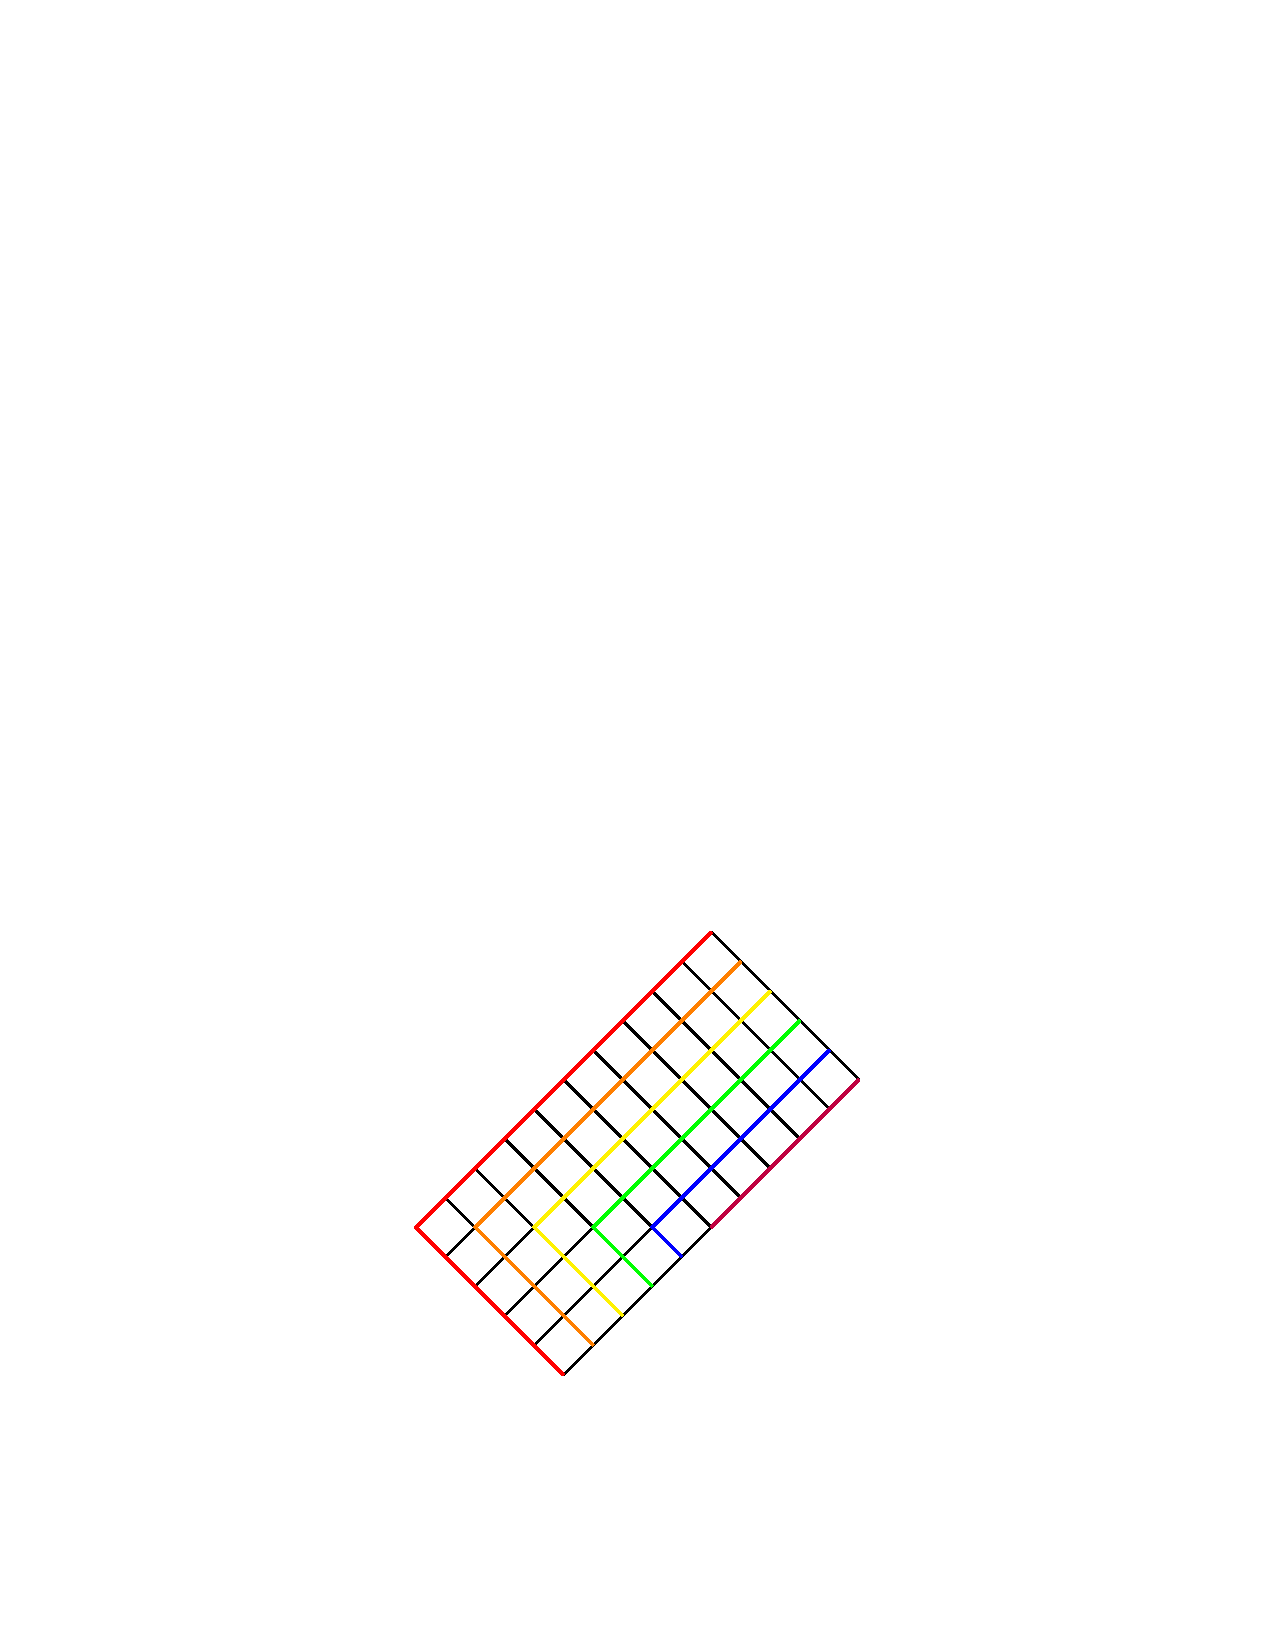
\includegraphics[width=8cm]{images/symchaindecomp.pdf}
	\end{figure}\parinf

Now for all $i\in[l]$ and  $j\in[z_i]$ then we have \begin{align*}
	\Rank(A_{i,1}\cup\{(j-1)\cdot k\})+(\Rank \lt(A_{i,k_i-j+1}\cup\{m_k\cdot k\}\rt)&= \Rank(A_{i,1})+(j-1)+\Rank(A_{i,k_i-j+1})+m_k\\
	& = \Rank(A_{i,1})+\Rank(A_{i,k_i})-(j-1)+m-k+(j-1)\\
	& = n+1-m_k+m_k=n+1
\end{align*}\parinn
Hence the new collection of chains $\mcA'=\{C_{i,j}\colon i\in[l],\ j\in[z_i]\}$ forms a symmetric chain decomposition of $B(m_1,\dots, m_k)$. Hence by mathematical induction we have the theorem.
\end{proof}
\subsection{General Lattices}

\dfn{Lattice}{A poset $U(,\leq)$ is a lattice $\forall\ x,y\in U$, then least upper bound of $x,y$, $x\vee y$  i.e. $$x\vee y\geq x,y\text{ and }\forall\ z\in U:\ z\geq x,y\implies z\geq x\vee y$$ also called \textit{join} of $x,y$ exists and the greatest lower bound of $x,y$, $x\wedge y$ i.e. $$x\wedge y\leq x,y\text{ and }\forall\ z\in U:\ z\leq x,y\implies z\leq x\wedge y$$ also called \textit{meet} of $x,y$ exists.}

\begin{Theorem}{Tarski's Fixed Point Theorem}{}
	Let $(U,leq)$ be a finite lattice and $f:U\to U$ be a monotone function (i.e. $x\leq\implies f(x)\leq f(y)$) then define $$z_{max}=\bigvee_{x\leq f(x)}x,\qquad z_{\min}=\bigwedge_{f(x)\leq x}x$$Then $z_{\max}$ is the largest fixed point and $z_{\\min}$ is the smallest fixed point.
\end{Theorem}
\begin{proof}
	Define the sets $$S_{\max}=\{x\in U\colon x\leq f(x)\}\qquad S_{\min}=\{x\in U\colon f()\leq x\}$$Now observe that $S_{\max}\neq \emptyset$ since $\min(U)\in S_{\max}$. And similarly $S_{min}\neq\emptyset$ as $\max(U)\in S_{\min}$. 
	
	Now $\forall\ x\in S_{\max}$ we   have $$x\leq z_{\max}\implies f(x)\leq f(z_{\max})\implies x\leq f(z_{\max})$$Now it follows that $$z_{\max}\leq f(z_{\max})\implies f(z_{\max})\leq f\lt(f(z_{\max})\rt)\implies f(z_{\max})\in S_{\max} \implies f(z_{\max})\leq z_{max}\implies z_{\max}=f(z_{\max})$$Therefore $z_{\max}$ is a fixed point. Now $z_{\max}$ is also largest fixed point since all the fixed points are in $S_{\max}$.
	
	Similarly we get that $z_{\min}$ is the fixed point and it is the smallest fixed point since all fixed points are in $S_{\min}$. Hence we have the theorem. 
\end{proof}
\begin{remark}
	Tarski's Fixed Point Theorem is not true for infinite lattices. For example take $U=\bbZ$ and take $f:\bbZ\to \bbZ$ where $f(n)=n^2+1$. Then $f$ has no fixed point.
\end{remark}
\section{Probabilistic Method}
The probabilistic method is a powerful tool for tackling many problems in discrete
mathematics. Roughly speaking, the method works as follows: trying to prove that
a structure with certain desired properties exists, one defines an appropriate prob-
ability space of structures and then shows that the desired properties hold in these
structures with positive probability.
\subsection{Ramsey Numbers}
\begin{Definition}{Ramsey Number}{}
	For $k>0$, the $\sR(k)$ is the smallest integer such that any graph with $\sR(k)$ vertices  has either a clique of size $k$ or an independent set of size $k$.
\end{Definition}
\begin{lemma}{}{}
	For all $k>4$, $\sR(k)>2^{\frac{k}2}$ i.e  $\exs$ a graph with $2^{\frac{k}2}$ vertices that does not have a $k$ size clique or $k$ size independent set.
\end{lemma}
\begin{proof}
	Let $n=2^{\frac{k}2}$ and consider a random graph (i.e. each edge appears with $\frac12$ probability) with $n$ vertices. Let $G$ be such a graph. We will show that $$\underset{G}{\bbP}[\exs\ S\subseteq [n]\colon |S|=k, \ S\text{ is not a clique or independent set}]<1$$Now using the union bound it is enough to show that $$\sum_{S\subseteq[n],\ |S|=k}\underset{G}{\bbP}[S\text{ is aa clique or independent set}]<1$$Now we have $$\sum_{S\subseteq[n],\ |S|=k}\underset{G}{\bbP}[S\text{ is aa clique or independent set}]=\sum_{S\subseteq[n],\ |S|=k}2\times \lt(\frac12\rt)^{\binom{k}2}=\binom{n}{k}\frac{2}{2^{\binom{k}2}}$$Hence it suffices to show that $$\binom{n}{k}\frac{2}{2^{\binom{k}2}}<1\iff 2\binom{n}k2^{-\frac{k^2-k}2}<1\iff \frac{\cancel{n^k}}{k!}\;\frac{2^\frac{k}2+1}{\cancel{2\st^{\frac{k^2}2}}}<1\iff\frac{2^{\frac{k}2+1}}{2^{\frac{k^2}2}}<1$$The last inequality is  true when $k> 4$.
	
	Hence when $k>4$ we have $\underset{G}{\bbP}[\exs\ S\subseteq [n]\colon |S|=k, \ S\text{ is a clique or independent set}]<1$. Hence $$\underset{G}{\bbP}[\forall\ S\subseteq [n]\colon |S|=k, \ S\text{ is not a clique or independent set}]>0$$Therefore there exists a graph $G$ with $2^{\frac{k}2}$ many vertices which does not have a $k$ size clique or $k$ size independent set. 
\end{proof}
\subsection{Turan's Theorem}
\begin{Theorem}{Turan's Theorem}{}
	Let $k>0$ and $G$ be a graph with $n$ vertices without a clique of size $k+1$. The number of edges in $G < \lt(1-\frac1k\rt)\frac{n^2}{2}$. 
\end{Theorem}
\begin{proof}
	We will show that if $|E|< \binom{n}2-\lt(1-\frac1k\rt)\frac{n^2}2$ then there is an independent set of size $k+1$. Then by flipping the graph i.e. taking the edge set which is  the complement of the edge set of $G'=(V,E)$ we get a clique of size $k+1$.
	
	Consider an uniformly random permutation of vertices $[n]$ and let $S$ be the set of vertices that occur before all their neighbors. Hence $S$ forms an independent set. Therefore we have $$\bbE[|S|]=\sum_{i\in[n]}\bbP[i\in S]=\sum_{i\in [n]}\frac1{d_i+1}$$Here the last step is true because the vertex $i$ has $d_i$ many neighbors and if we arrange all the neighbors and the vertex $i$ one after another what is the probability the vertex $i$ comes at first among them. 
	
	Now by Jensen Inequality we have $$\bbE[|S|]=\sum_{i\in[n]}\frac{1}{d_i+1}\geq \frac{n}{\frac1n\lt(\sum\limits_{i\in[n]}d_i\rt)+1}=\frac{n}{\frac2n|E|+1}=\frac{n^2}{2|E|+n}$$Since  $|E|< \binom{n}2-\lt(1-\frac1k\rt)\frac{n^2}2=\frac{n(n-1)}2-\lt(1-\frac1k\rt)\frac{n^2}2=\frac12\lt(\frac{n^2}k-n\rt)$. Therefore we have $$\bbE[|S|]\geq \frac{n^2}{2|E|+n}>\frac{n^2}{\frac{n^2}k-n+n}=k$$Hence $\bbE[|S|]>k$ and since $|S|$ is always a positive integer we have $\bbE[|S|]\geq k+1$. Since the average cannot exceed the maximum we have the largest independent set has size at least $k+1$. Therefore if we take the complement graph there is a $k+1$ size clique. Hence
	
	Hence if we have $|E|\geq \binom{n}2-\lt(1-\frac1k\rt)\frac{n^2}2$ there is no independent set of size $k+1$. And therefore the complement graph also has no clique of size $k+1$.
\end{proof}

\subsection{Magnitude of Boolean Quadratic Forms}
\begin{lemma}{Magnitude of Boolean Quadratic Forms}{}
	Let $n>0$ and $a_{i,j}\in\{1,-1\}$ for all $i,j\in[n]$. Then $$\max_{x_1,\dots, x_n\in \{1,-1\}}\max_{y_1,\dots, y_n\in \{1,-1\}}\sum_{i,j\in[n]}a_{i,j}x_iy_j\geq \Om\lt(n^{1.5}\rt)$$
\end{lemma}
\begin{proof}
	Let $B$ denote the $LHS$ of given expression i.e. $$B\coloneqq \max_{x_1,\dots, x_n\in \{1,-1\}}\max_{y_1,\dots, y_n\in \{1,-1\}}\sum_{i,j\in[n]}a_{i,j}x_iy_j$$Now\begin{align*}
		B& = \max_{x_1,\dots, x_n\in \{1,-1\}}\max_{y_1,\dots, y_n\in \{1,-1\}}\sum_{i,j\in[n]}a_{i,j}x_iy_j\\
		& = \max_{x_1,\dots, x_n\in \{1,-1\}}\max_{y_1,\dots, y_n\in \{1,-1\}}\sum_{j=1}^ny_j\sum_{i=1}^n a_{i,j}x_i\\
		& =  \max_{x_1,\dots, x_n\in \{1,-1\}}\sum_{j=1}^n\max_{y_1,\dots, y_n\in \{1,-1\}}y_j\sum_{i=1}^n a_{i,j}x_i\\
		& = \max_{x_1,\dots, x_n\in \{1,-1\}}\sum_{j=1}^n\lt|\sum_{i=1}^n a_{i,j}x_i\rt|\\
	\end{align*}Now it is enough to show that $$\underset{X_1,\dots, X_n}{\bbE}\lt[\sum_{j=1}^n\lt|\sum_{i=1}^na_{i,j}X_i\rt|\rt] =\sum_{j=1}^n\underset{X_1,\dots, X_n}{\bbE}\lt[ \lt|\sum_{i=1}^na_{i,j}X_i \rt| \rt]  \geq \Om(n^{1.5})\implies \underset{X_1,\dots, X_n}{\bbE}\lt[ \lt|\sum\limits_{i=1}^na_{i,j}X_i \rt| \rt] \geq \Om(n^{0.5})$$Now in the expression $\underset{X_1,\dots, X_n}{\bbE}\lt[ \lt|\sum\limits_{i=1}^na_{i,j}X_i \rt| \rt] $ the $a_{i,j}$ doesn't matter as they take the values of $1$ or $-1$ and $X_i$ also takes the values $1$ or $-1$ we can think $Y_i=a_{i,j}X_i$ where $Y_i $ takes values $1$ or $-1$. Then we have $$\underset{X_1,\dots, X_n}{\bbE}\lt[ \lt|\sum\limits_{i=1}^na_{i,j}X_i \rt| \rt]=\underset{Y_1,\dots, Y_n}{\bbE}\lt[ \lt|\sum\limits_{i=1}^nY_i \rt| \rt]=\frac1{2^n}\sum_{k=0}^n\binom{n}{k}|2k-n|$$ Now we have 
\begin{align*}
	\sum_{k=0}^n\binom{n}k|n-2k|&=2\sum_{k=0}^{\lfloor n/2\rfloor}\binom{n}k(n-2k)=2\left(n\sum_{k=0}^{\lfloor n/2\rfloor}\binom{n}k-2\sum_{k=0}^{\lfloor n/2\rfloor}k\binom{n}k\right)\\\\
	&=2n\left(\sum_{k=0}^{\lfloor n/2\rfloor}\binom{n}k-2\sum_{k=0}^{\lfloor n/2\rfloor}\binom{n-1}{k-1}\right)=2n\left(\sum_{k=0}^{\lfloor n/2\rfloor}\left(\binom{n}k-\binom{n-1}{k-1}\right)-\sum_{k=0}^{\lfloor n/2\rfloor}\binom{n-1}{k-1}\right)\\\\
	&=2n\left(\sum_{k=0}^{\lfloor n/2\rfloor}\binom{n-1}k-\sum_{k=0}^{\lfloor n/2\rfloor}\binom{n-1}{k-1}\right)=2n\left(\sum_{k=0}^{\lfloor n/2\rfloor}\binom{n-1}k-\sum_{k=0}^{\lfloor n/2\rfloor-1}\binom{n-1}k\right)=2n\binom{n-1}{\lfloor n/2\rfloor}=\Om(n^{0.5})
\end{align*}Hence we have $\underset{X_1,\dots, X_n}{\bbE}\lt[ \lt|\sum\limits_{i=1}^na_{i,j}X_i \rt| \rt]=\Om(n^{0.5})$. Therefore $B\geq \Om(n^{1.5})$.
\end{proof}
\subsection{Lov\'{a}sz-Local Lemma}
Now we will prove a very strong result called the Lov\'{a}sz-Local Lemma. But before that first we need the define Dependency Graph of finite set of events.
\begin{Definition}{Dependency (di)graph}{}
	Let $E_1,\dots, E_n$ be events. For each $i$ there is some subset $N(i)\subseteq [n]$ such that $A_i$ is independent from $\{A_j\colon j\notin N(i)\cup \{i\}\}$. Here event $A$ is independent from $\{B_1,\dots, B_k\}$ means $A$ is independent of every event of the form $\bigwedge\limits_{i=1}^kC_i$ where $C_i$ is either $B_i$ or $\ovB_i$.\parinn
	
	We can represent the above relations by the Dependency Graph which is a directed whose vertices is $[n]$ and the set of neighbors of $i\in[n]$  is the set $N(i)$.
\end{Definition}
\begin{Theorem}{Lov\'{a}sz-Local Lemma}{}
	Let $E_1,\dots, E_n$ be events and $G=([n],E)$ be the dependency graph of these events. Suppose $x_1,\dots, x_n$ satisfy $$\forall i\in[n]\quad \bbP[E_i]\leq x_i\prod_{j:(i,j)\in E}(1-x_j)$$Then $$\bbP\lt[\bigwedge_{i=1}^n\ov{E}_i\rt]\geq \prod_{i=1}^n(1-x_i)$$
\end{Theorem}
\begin{proof}
	We will first prove the following claim:\begin{claimwidth}
		\begin{claim}{}{}
			$\forall\ i\in[n]$ and $\forall\ S\subseteq[n]$, $i\notin S$ we have $$\bbP\lt[E_i\mid \bigwedge_{j\in S}\ovE_j\rt]\leq\frac{\bbP[E_i]}{\prod\limits_{j\in S,\ (i,j)\in E}(1-x_j)}$$
		\end{claim}
	\begin{proof}
		We will prove this using induction on $|S|$. For base case let $S=\emptyset$. Then $S\cap\{j\colon (i,j)\in E\}=\emptyset$. Then $\prod\limits_{j\in S,\ (i,j)\in E}(1-x_j)=1$. And since $S$ in empty $\bbP\lt[E_i\mid \bigwedge\limits_{j\in S}\ovE_j\rt]=\bbP[E_i]$. Therefore the base case follows. \parinn
		
		Suppose $|S|=k$. If $S\cap\{j\colon (i,j)\in E\}=\emptyset$, $E_i$ is independent of $E_j$ for all $j\in S$. Therefore $\bbP\lt[E_i\mid \bigwedge\limits_{j\in S}\ovE_j\rt]=\bbP[E_i]$. Also since $S\cap\{j\colon (i,j)\in E\}=\emptyset$ we have $\prod\limits_{j\in S,\ (i,j)\in E}(1-x_j)=1$. Therefore the claim follows.
		
		Now Suppose $S\cap\{j\colon (i,j)\in E\}\neq\emptyset$. Let $S_1\coloneqq S\cap\{j\colon (i,j)\in E\}$ and $S_2\coloneqq S\setminus S_1$. Then we have $$\bbP\lt[E_i\mid \bigwedge_{j\in S}\ov{E}_j\rt]=\frac{\bbP\lt[ E_i\wedge \lt( \bigwedge\limits_{j\in S_1}\ovE_j\rt)\mid \bigwedge\limits_{j\in S_2}\ovE_j \rt]}{\bbP\lt[  \bigwedge\limits_{j\in S_1}\ovE_j\mid \bigwedge\limits_{j\in S_2}\ovE_j \rt]}\leq \frac{\bbP\lt[ E_i\mid \bigwedge\limits_{j\in S_2}\ovE_j \rt]}{\bbP\lt[  \bigwedge\limits_{j\in S_1}\ovE_j\mid \bigwedge\limits_{j\in S_2}\ovE_j \rt]}\leq\frac{\bbP[ E_i]}{\bbP\lt[  \bigwedge\limits_{j\in S_1}\ovE_j\mid \bigwedge\limits_{j\in S_2}\ovE_j \rt]} $$So we will now give a lower bound on $\bbP\lt[  \bigwedge\limits_{j\in S_1}\ovE_j\mid \bigwedge\limits_{j\in S_2}\ovE_j \rt]$. Now we have \begin{align*}
			\bbP\lt[  \bigwedge\limits_{j\in S_1}\ovE_j\mid \bigwedge\limits_{j\in S_2}\ovE_j \rt] & = \prod_{k\in S_1}\bbP\lt[ E_k\ \lt|\ \ \lt(\bigwedge_{j\in S_2}\ovE_j\rt) \wedge \lt( \bigwedge_{j<k,\ j\in S_1}\ovE_j\rt) \rt.  \rt]\\
			& \geq \prod_{k\in S_1} \lt(1-\frac{\bbP[E_k]}{\prod\limits_{\substack{j\in S_2\\ (k,j)\in E}}(1-x_k)  \prod\limits_{\substack{j\in S_1,\, j<k\\ (k,j)\in E}}(1-x_k)  }   \rt) &[\text{Inductive Hypothesis}]\\
			& \geq \prod_{k\in S_1}(1-x_k)& \lt[\bbP[E_k]\leq x_k\prod_{j:(k,j)\in E}(1-x_j)\rt]
		\end{align*}Therefore we have $$\bbP\lt[E_i\mid \bigwedge_{j\in S}\ovE_j\rt]\leq \frac{\bbP[E_i]}{\prod\limits_{k\in S_1}(1-x_k)}=\frac{\bbP[E_i]}{\prod\limits_{k\in S,(i,k)\in E}(1-x_k)}$$Hence we have the claim	\end{proof}
	\end{claimwidth}
Now using the claim we have $$\bbP\lt[ \bigwedge_{i=1}^n\ovE_i \rt]=\prod_{i=1}^n\bbP\lt[ \ovE_i\mid\bigwedge_{j<i}\ovE_j \rt]$$
\end{proof}

Using Lova\'{a}sz Local Lemma we have the following corollary:
\begin{corolary}{}{}
	Suppose $G$ has degree $\leq d$ and $x_1=x_2=\cdots=x_n=\frac1{d+1}$. If $\forall\ i\in[n]$ $$\bbP[E_i]\leq\frac{1}{e(d+1)}\implies \bbP\lt[\bigwedge_{i=1}^n\ov{E}_i\rt]>0$$
\end{corolary}
\dfn{Negative Dependency (di)graph}{
$G$ is a negatve dependency (di)graph if for every event $E_i$ and every subset $S\subseteq [n]\setminus N(i)\cup\{i\}$ we have $$\bbP\lt[E_i\cap\bigcup_{j\in S}E_j   \rt]\geq \bbP[E_i]\bbP\lt[ \bigcup_{j\in S}E_j \rt]$$ 
}
\begin{Theorem}{Lopsided Lov\'{a}sz Local Lemma}{}
	Suppose $G$ is a negative dependency (di)graph for events $E_1,\dots, E_n$ and there exists $x_1,\dots, x_n$ which satisfy $$\forall i\in[n]\quad \bbP[E_i]\leq x_i\prod_{j:(i,j)\in E}(1-x_j)$$Then $$\bbP\lt[\bigwedge_{i=1}^n\ov{E}_i\rt]\geq \prod_{i=1}^n(1-x_i)$$
\end{Theorem}
\begin{proof}
	content...
\end{proof}
\section{Linear Algebraic Techniques in Combinatorics}
\subsection{Odd Town Even Town}
\begin{lemma}{}{}
	Let $\mcF\subseteq 2^{[n]}$ be such that $|A|$ is odd for every $A\in \mcF$ and $|A\cap B|$ is even for every distinct $A,B\in \mcF$. Then $|\mcF|\leq n$.
\end{lemma}
\begin{proof}
	Define $x_A$ for every $A\in \mcF$ to be the characteristic vector in $\{0,1\}^n$ where $x_A(i)=1\iff i\in A$. We will show that $x_A$'s for all $A\in\mcF$ are linearly independent over $|bbF_2$. This suffices to show that $|\mcF\leq n$ since $$|\mcF|=|\{x_A\colon A|\in\mcF\}|\leq \dim_{\bbF_2} \{0,1\}^n=n$$
\end{proof}
\begin{lemma}{}{}
	Let $\mcF\subseteq 2^{[n]}$ be such that $|A|$ is even for every $A\in \mcF$ and $|A\cap B|$ is off for every distinct $A,B\in \mcF$. Then $|\mcF|\leq n$
\end{lemma}
\subsection{Fisher's Inequality}
\begin{Theorem}{Fisher's Inequality}{}
	Suppose that $\mcF\subseteq 2^{[n]}$ is a family of nonempty clubs such that for some fixed $k$, $|A\cap B|=k$ for every distinct $A,B\in \mcF$. Then $|\mcF|\leq n$.
\end{Theorem}
\subsection{RW Theorem}
\section{Projective Planes}

\end{document}
